%
\documentclass[12pt]{article}
% Oct 26, 1999
\setlength{\oddsidemargin}{-0.125in}
\setlength{\topmargin}{-0.5in} \setlength{\textwidth}{6.5in}
\setlength{\textheight}{9in}

\setlength{\textheight}{9in} \setlength{\textwidth}{6.5in}
\setlength{\topmargin}{-40pt} \setlength{\oddsidemargin}{0pt}
\setlength{\evensidemargin}{0pt}

\setlength{\textheight}{8.5in} \setlength{\textwidth}{6.5in}
\setlength{\topmargin}{-36pt} \setlength{\oddsidemargin}{0pt}
\setlength{\evensidemargin}{0pt} \tolerance=500
\renewcommand{\baselinestretch}{1.5}
%\input psfig.tex
\usepackage{amssymb}
\usepackage{amsmath}
\usepackage{latexsym}
\usepackage{array}
\usepackage{morefloats}
\usepackage{epsfig}
\usepackage{rotating}
\usepackage{graphicx}
\usepackage{subfigure}
\usepackage{url}
\usepackage{mathtools}
\usepackage{enumerate}
\usepackage{wasysym}
\usepackage{threeparttable}
\usepackage{lscape}
\usepackage{natbib}
\usepackage{color}
\usepackage{epstopdf}
\usepackage{hyperref}
\usepackage{bm, bbm}

\newcommand{\mbv}[1]{\mbox{\boldmath$#1$\unboldmath}}
\newcommand{\mbf}[1]{\mathbf{#1}}
\newcommand{\iid}{\stackrel{\mathrm{iid}}{\sim}}
\newcommand{\mcal}[1]{\mathcal{#1}}
\newcommand{\bl}{\color{blue}}
\newcommand{\gr}{\color{green}}
\newcommand{\rd}{\color{red}}
\newcommand{\blk}{\color{black}}
\newcommand{\mbb}[1]{\mathbb{#1}}
\newtheorem{theorem}{Theorem}[section]
\newtheorem{lemma}[theorem]{Lemma}
\newtheorem{proposition}[theorem]{Proposition}
\newtheorem{corollary}[theorem]{Corollary}

\newenvironment{proof}[1][Proof]{\begin{trivlist}
\item[\hskip \labelsep {\bfseries #1}]}{\end{trivlist}}
\newenvironment{definition}[1][Definition]{\begin{trivlist}
\item[\hskip \labelsep {\bfseries #1}]}{\end{trivlist}}
\newenvironment{example}[1][Example]{\begin{trivlist}
\item[\hskip \labelsep {\bfseries #1}]}{\end{trivlist}}
\newenvironment{remark}[1][Remark]{\begin{trivlist}
\item[\hskip \labelsep {\bfseries #1}]}{\end{trivlist}}

\newcommand{\qed}{\nobreak \ifvmode \relax \else
      \ifdim\lastskip<1.5em \hskip-\lastskip
      \hskip1.5em plus0em minus0.5em \fi \nobreak
      \vrule height0.75em width0.5em depth0.25em\fi}


%%%%%%%%%%%%%%%%%%%%%%%%%%%%%%%%%%%%%%%%%%
\def\wt{\widetilde}
\def\diag{\hbox{diag}}
\def\wh{\widehat}
\def\AIC{\hbox{AIC}}
\def\BIC{\hbox{BIC}}
%- Makes the section title start with Appendix in the appendix environment
\newcommand{\Appendix}
{%\appendix
\def\thesection{Appendix~\Alph{section}}
%\def\thesubsection{\Alph{section}.\arabic{subsection}}
\def\thesubsection{A.\arabic{subsection}}
}
\def\diag{\hbox{diag}}
\def\log{\hbox{log}}
\def\bias{\hbox{bias}}
\def\Siuu{\boldSigma_{i,uu}}
\def\ANNALS{{\it Annals of Statistics}}
\def\BIOK{{\it Biometrika}}
\def\whT{\widehat{\Theta}}
\def\STATMED{{\it Statistics in Medicine}}
\def\STATSCI{{\it Statistical Science}}
\def\JSPI{{\it Journal of Statistical Planning \& Inference}}
\def\JRSSB{{\it Journal of the Royal Statistical Society, Series B}}
\def\BMCS{{\it Biometrics}}
\def\COMMS{{\it Communications in Statistics, Theory \& Methods}}
\def\JQT{{\it Journal of Quality Technology}}
\def\STIM{{\it Statistics in Medicine}}
\def\TECH{{\it Technometrics}}
\def\AJE{{\it American Journal of Epidemiology}}
\def\JASA{{\it Journal of the American Statistical Association}}
\def\CDA{{\it Computational Statistics \& Data Analysis}}
\def\dfrac#1#2{{\displaystyle{#1\over#2}}}
\def\VS{{\vskip 3mm\noindent}}
\def\boxit#1{\vbox{\hrule\hbox{\vrule\kern6pt
          \vbox{\kern6pt#1\kern6pt}\kern6pt\vrule}\hrule}}
\def\refhg{\hangindent=20pt\hangafter=1}
\def\refmark{\par\vskip 2mm\noindent\refhg}
\def\naive{\hbox{naive}}
\def\itemitem{\par\indent \hangindent2\parindent \textindent}
\def\var{\hbox{var}}
\def\cov{\hbox{cov}}
\def\corr{\hbox{corr}}
\def\trace{\hbox{trace}}
\def\refhg{\hangindent=20pt\hangafter=1}
\def\refmark{\par\vskip 2mm\noindent\refhg}
\def\Normal{\hbox{Normal}}
\def\povr{\buildrel p\over\longrightarrow}
\def\ccdot{{\bullet}}
\def\be{\begin{eqnarray}}
\def\ee{\end{eqnarray}}
\def\bq{\begin{equation}}
\def\eq{\end{equation}}
\def\bse{\begin{eqnarray*}}
\def\ese{\end{eqnarray*}}
\def\pr{\hbox{pr}}
\def\wh{\widehat}
\def\trans{^{\rm T}}
\def\myalpha{{\cal A}}
\def\th{^{th}}
\def\bs{\mathbf{s}}

\DeclarePairedDelimiter\ceil{\lceil}{\rceil}
\DeclarePairedDelimiter\floor{\lfloor}{\rfloor}


\DeclareMathOperator{\vect}{vec}
\DeclareMathOperator{\vech}{vech}

\newtheorem{alg}{Algorithm}

%%%%%%%%%%%%%%%%%%%%%%%%%%%%%%%%%%%%%
\begin{document}
\thispagestyle{empty} \baselineskip=28pt

\thispagestyle{empty} \baselineskip=28pt

%
\begin{center}
%{\LARGE{\bf Supplemental Web Material: Particle Swarm Optimization Assisted Metropolis Hastings Algorithms}}
{\LARGE{\bf Particle Swarm Optimization Assisted Metropolis Hastings Algorithms}}
\end{center}


\baselineskip=12pt


%%
%%
%%
%%%%%%%%%%%%%%%%%%%%%%%%%%%%%%%%%%%%%%%%%%%%%%%%%%%%%%%%%%%%%%%%%%%%%%%%
\vskip 2mm
\begin{center}
Matthew Simpson,\footnote{(\baselineskip=10pt to whom correspondence should be addressed)
Department of Statistics, University of Missouri,
146 Middlebush Hall, Columbia, MO 65211-6100, themattsimpson@gmail.com}
% Christopher K. Wikle,\footnote{\label{note:aff}\baselineskip=10pt
% Department of Statistics, University of Missouri,
% 146 Middlebush Hall, Columbia, MO 65211-6100}
% and Scott H. Holan\textsuperscript{\ref{note:aff}}
\end{center}
\clearpage\pagebreak\newpage \pagenumbering{arabic}

\baselineskip=24pt


\section*{Comparing AT-BBPSO, BBPSO, and PSO algorithms}\label{sec:psocompare}
\begin{appendix}
\Appendix    % This makes the section title start with Appendix!
\renewcommand{\theequation}{A.\arabic{equation}}
\setcounter{equation}{0}
In order to compare AT-BBPSO to other PSO variants, we employ a subset of test functions used in \citet{hsieh2010modified}. Each function is listed in Table \ref{tab:testfuns} along with the global maximum and argmax, and the initialization range for the simulations. Further description of many of these functions can be found in \citet{clerc2010particle}. Each function is randomly initialized in a range that does not contain its global maximum.

\begin{table}[h]
\centering
\begin{tabular}{llll}
 Equation & ArgMax & Maximum & Initialization \\\hline
 $Q_1(\bm{\theta}) = -\sum_{i=1}^D\theta_i^2$ & $\bm{\theta}^* = \bm{0}$ & $Q_1(\bm{\theta}^*) = 0$  & $(50, 100)^D$ \\
 $Q_2(\bm{\theta}) = -\sum_{i=1}^D\left(\sum_{j=1}^i \theta_j\right)^2 $ & $\bm{\theta}^* = \bm{0}$ & $Q_2(\bm{\theta}^*) = 0$ & $(50, 100)^D$ \\
% $Q_3(\bm{\theta}) = -0.5 - \frac{\sin(||\bm{\theta}||) - 0.5}{\left(1 + 0.001||\bm{\theta}||^2\right)^2}$ & $\left\{||\bm{\theta}^*|| \approx 4.6849\right\}$ & $Q_3(\bm{\theta}^*) \approx 0.9358$ & $(50, 100)^D$ \\ 
 $Q_3(\bm{\theta}) = -\sum_{i=1}^{D-1}\left[100\{\theta_{i+1} + 1 - (\theta_i + 1)^2\} + \theta_i^2\right]$ & $\bm{\theta}^* = \bm{0}$ & $Q_3(\bm{\theta}^*) = 0$ & $(15, 30)^D$ \\
 $Q_4(\bm{\theta}) = 9D - \sum_{i=1}^D\{\theta_i^2 - \cos(2\pi \theta_i) + 10\}$ & $\bm{\theta}^*=\bm{0}$ & $Q_4(\bm{\theta}^*) = 0$ & $(2.56, 5.12)^D$ \\
 %$Q_6(\bm{\theta}) = \sum_{i=1}^D\theta_i\sin\left(\sqrt{|\theta_i|}\right)$ & None & None & $(-500, -250)^D$ \\
 $Q_5(\bm{\theta}) = -\frac{1}{4000}||\bm{\theta}||^2 + \prod_{i=1}^D\cos\left(\frac{\theta_i}{\sqrt{i}}\right) - 1$ & $\bm{\theta}^* = \bm{0}$ & $Q_5(\bm{\theta}^*) = 0$ & $(300, 600)^D$ \\
 \shortstack[l]{$Q_6(\bm{\theta}) = 20\exp\left(-0.2\sqrt{\frac{1}{D}||\bm{\theta}||}\right)$ \\ \ \ \ \ \ \ \ \ $+ \exp\left\{\frac{1}{D}\sum_{i=1}^D\cos(2\pi \theta_i)\right\} - 20 - \exp(1)$} & $\bm{\theta}^* = \bm{0}$ & $Q_6(\bm{\theta}^*) = 0$ & $(16, 32)^D$\\\hline
\end{tabular}
\caption{Test functions for evaluating PSO algorithms. The dimension of $\bm{\theta}$ is $D$ and $||.||$ is the Euclidean norm: $||\bm{\theta}|| = \sqrt{\sum_{i=1}^D\theta_i^2}$.} 
\label{tab:testfuns}
\end{table}

We use several PSO algorithms in the simulation study. The standard PSO algorithm uses the parameter values suggested by \cite{blum2008swarm} and \cite{clerc2002particle}. The AT-BBPSO variants are implemented a wide variety of parameter values, but all have the scale parameter initialized at $\sigma(0)=1$, and both increment or decrement $\log\sigma$ by $c=0.1$ every iteration. The AT-PSO variants are initialized at $\omega(0)=1$ and $\log\omega$ is incremented or decremented by $c=0.1$ every iteration. In addition, each algorithm is implemented using each of three neighborhood structures. The global neighborhood allows each particle to look at each other particle in the swarm in order to determine its group best --- in this case the group best is the swarm best and is used by all particles. The ring-1 neighborhood only allows particles to look at their neighbors as defined by a ring structure. Label each particle with an integer, $0, 1, \dots, n-1$. Then particle $i$ only looks at particles $i-1$ mod $n$ and $i+1$ mod $n$ in order to determine what its group best is. Addition and subtraction is mod $n$ so that particle $0$ looks at particles $n-1$ and $1$ to determine its group best. This restricts the flow of information across particles allowing them to explore their nearby space more fully before being pushed in the direction of the rest of the swarm. For less well behaved functions this behavior typically improves the algorithm's ability to find the global max by allowing for more exploration of the objective surface and less exploitation of the best known information. Finally the ring-3 neighborhood is similar to ring-1 but allows each particle to look at its 3 nearest neighbors in each direction, so, for example, particle 1 sees particles 2, 3, 4, $n_{swarm}$, $n_{swarm} -1$, and $n_{swarm}-2$. This still restricts the flow of information across the swarm, but less so than the ring-1 neighborhood. 

Each algorithm was used to optimize each objective function for 500 iterations over 100 replications. Initializations were changed across replications but held constant across algorithms. The standard PSO, DI-PSO, and AT-PSO algorithms initialized their velocity terms with $v_{ij}(0)\stackrel{iid}{\sim}U(-1,1)$. Tables \ref{tab:psosim1}-\ref{tab:psosim6} contain the simulation results for objective functions 1-6 respectively (OF1, OF2, etc.). We use several measures to quantify how well each algorithm finds the global maximum. First, each table includes the mean and standard deviation of the absolute difference between the true global maximum and the algorithm's estimated global maximum across all 50 replication. Second, each table includes measures of two convergence criterion --- the proportion of the replications that came within $0.01$ of the true global maximum and the proportion that came with $0.0001$, denoted by $\widehat{p}_2$ and $\widehat{p}_4$ respectively. 

We highlight only some of the features of these tables. First, the BBPSO-MC and AT-BBPSO-MC almost always do worse than their BBPSOxp-MC and AT-BBPSOxp-MC cousins, both in terms of mean absolute difference from the global maximum and in terms of the convergence criterion. The main exception is OF2. Second, for most algorithms the more restrictive neighborhood appears to be result in algorithms which do a better job of finding the global max. This is not universally true, and one interesting class of exceptions are the AT-PSO algorithms. For them, it appears that the target improvement rate ($R^*$) and the neighborhood interact. When the rate is high a more restrictive neighborhood is preferable, while when the rate is low a less restrictive neighborhood is preferable. Though for OF4 a more restrictive neighborhood always seems preferable. Typically, the AT-PSO algorithms with $R^*=0.3$ or $R^*=0.5$ using the ring-1 neighborhood does the best of the AT-PSO algorithms, though there are exceptions.

For the DI-PSO algorithms often there is a parameter-neighborhood combination that does well, typically from setting $\alpha=200$ (20\% of the 500 iterations) and $\beta=1$ and using either the ring-1 or ring-3 neighborhood. Call this combination with the ring-1 neighborhood the default DI-PSO algorithm. The default combination typically does the best of all the DI-PSO algorithms but they can sometimes still do much worse than the best alternatives (e.g., for OF2). In the AT-BBPSO algorithms, lower values of $df$ often result in better algorithms, though sometimes the difference is small. The impact of $R^*$ is much smaller, though $R^*=0.3$ or $R^*=0.5$ seem to be the safest choices, though other classes of algorithms will often perform better. 

In general, the standard PSO algorithm and the BBPSOxp-MC algorithm do pretty well and should serve as baselines, typically using the ring-1 neighborhood. For OF1, PSO meets both convergence criterion 100\% of the time in our simulations, while only BBPSOxp-MC has $\widehat{p}_2=1$. None of the AT-BBPSOxp-MC algorithms are able to hit the second criterion at a high rate, though our recommended DI-PSO and AT-PSO algorithms are able to. For OF2, the standard PSO algorithm using the ring-3 neighborhood is the best performing of the baseline algorithms, with $\widehat{p}_2=0.86$ and $\widehat{p}_4=0.1$. The best performing algorithm overall is AT-PSO with $R^*=0.3$, yielding $\widehat{p}_2=\widehat{p}_4=1$, and AT-PSO with $R^*=0.5$ is in a close second with $\widehat{p}_2=1$ and $\widehat{p}_4=0.72$. None of the AT-BBPSO or DI-PSO algorithms even come close to the baseline. OF3 is much more challenging and almost no algorithm has nonzero convergence rates. The best baseline algorithm is BBPSOxp-MC with the ring-1 neighborhood, with a mean absolute difference from the true max of 18.77 respectively. The ring-1 PSO algorithm has a mean of 25.95, which we will use as another baseline for this objective function. Many of the ring-1 AT-BBPSOxp-MC algorithms are competitive with the baselines, but essentially nothing else is in terms of mean absolute difference. However, the ring-1 AT-PSO algorithm with $R^*=0.5$ does meet both convergence criterion in 2\% of replication, while no other algorithm ever meets the criterion. 

The best baseline algorithm for OF4 may be ring-1 PSO, with a mean absolute difference of 0.13 and convergence proportions of 0.90 and 0.86. However, the BBPSOxp-MC algorithm is comparable with a mean of 0.01 and $\widehat{p}_2=0.86$, but $\widehat{p}_4=0$. Which is better depends on how precise you need to estimate the global maximum. All of the AT-BBPSOxp-MC algorithms are similar to BBPSOxp-MC with a near zero mean, $\widehat{p}_2$ approaching 1 and $\widehat{p}_4$ essentially 0. None of the DI-PSO algorithms are competitive and even the best AT-PSO algorithms are worse than the baseline PSO algorithm. OF5 is another difficult one where most algorithms never meet any of the convergence criterion. ring-1 PSO and ring-3 PSO are the best baselines with mean absolute differences of 0.06 and 0.07 respectively. With the ring-1 or ring-3 neighborhood, AT-BBPSOxp-MC algorithms with $df=1$ are comparable to both baselines, The best performing algorithms in terms of mean absolute difference are the ring-1 AT-PSO algorithms with $R^*=0.3$ or $0.5$. OF6 is the most difficult with many local optima. The baseline algorithms do poorly, though ring-3 PSO and ring-1 PSO have high convergence proportions despite high mean absolute differences. The AT-BBPSOxp-MC algorithms with $df=1$ and $R^*=0.3$ or $0.5$ do much better in terms of the mean absolute difference, but almost never meet the convergence criterion. The ring-3 DI-PSO algorithm with $\alpha=200$ and $\beta=1$ is the best converging algorithm, with $\widehat{p}_2=0.7$ and $\widehat{p}_4=0.68$, though ring-3 AT-PSO with $R^*=0.1$ has $\widehat{p}_2=0.7$ and $\widehat{p}_4=0.12$

In general ring-1 or ring-3 PSO is a great baseline algorithm that works reasonably well over a wide variety of circumstances. The AT-BBPSOxp-MC algorithms with $df=1$ and $R^*=0.3$ or $0.5$ also tend to do reasonably well, though their strength seems to be in finding the region around the global max quickly. When the optimization problem is not too difficult, the best AT-BBPSOxp-MC algorithms have trouble converging as fast as the best alternatives, but when the optimization problem is difficult enough that convergence is unlikely in the number of allotted iterations AT-BBPSOxp-MC often gets closer to the global maximum than the alternatives on average.

The DI-PSO and AT-PSO algorithms similar conceptually, but often yield very different results. DI-PSO deterministically reduces the inertia parameter over time in the same manner given a fixed set of parameter values ($\alpha$ and $\beta$), while AT-PSO dynamically adjusts the inertia parameter to hit a target improvement rate. Figure \ref{fig:inertia} plots the inertia over time for the DI-PSO algorithm with $\alpha=200$, i.e. 20\% of the total number of PSO iterations, and $\beta=1$, and observed inertia over time for one replication of the $AT-PSO$ algorithm with target rate $R^*=0.5$ and ring-1 neighborhood for OF1 and one replication for OF8. All three algorithms have an initial inertia of $\omega(0)=1$. While DI-PSO smoothly decreases its inertia with a slowly decreasing rate, for OF1 AT-PSO very quickly drops its inertia to about 0.5 then bounces around around that point. It also jumps up above 1 initially, imploring the particles to cast a wider net in search of higher value areas of the search space. This is pretty typical behavior for the inertia parameter of AT-PSO --- it tends to bounce around a level which is approximately the average over time of the DI-PSO's inertia, though lower values of $R^*$ will result in higher inertias. In this way, AT-PSO alternates periods of search (relatively high inertia) and periods of exploitation (relatively low inertia). The main exception to this pattern is when AT-PSO converges around a local maximum. In this case, inertia plummets to zero as the particles settle down. This is precisely what happens for OF6 in Figure \ref{fig:inertia}, though in this case the maximum is not global --- Table \ref{tab:psosim6} indicates that ring-1 AT-PSO with $R^*=0.5$ very rarely converged to the global max. In optimization problems with multiple local optima, both AT-PSO and AT-BBPSO variants can exhibit this behavior prematurely converge to a local optima, so they may not be advantageous for those problems. Reducing the target improvement rate ($R^*$) can ameliorate this problem though. We used $c=0.1$ for all AT type algorithms in this section, but decreasing $c$ will slow down how fast the inertia parameter is adapted in AT-PSO algorithms and allow for a longer high inertia exploration phase, mimicing the DI-PSO algorithms to some extent. This may also help in problems with many local optima.

\begin{figure}[!ht]
\centering
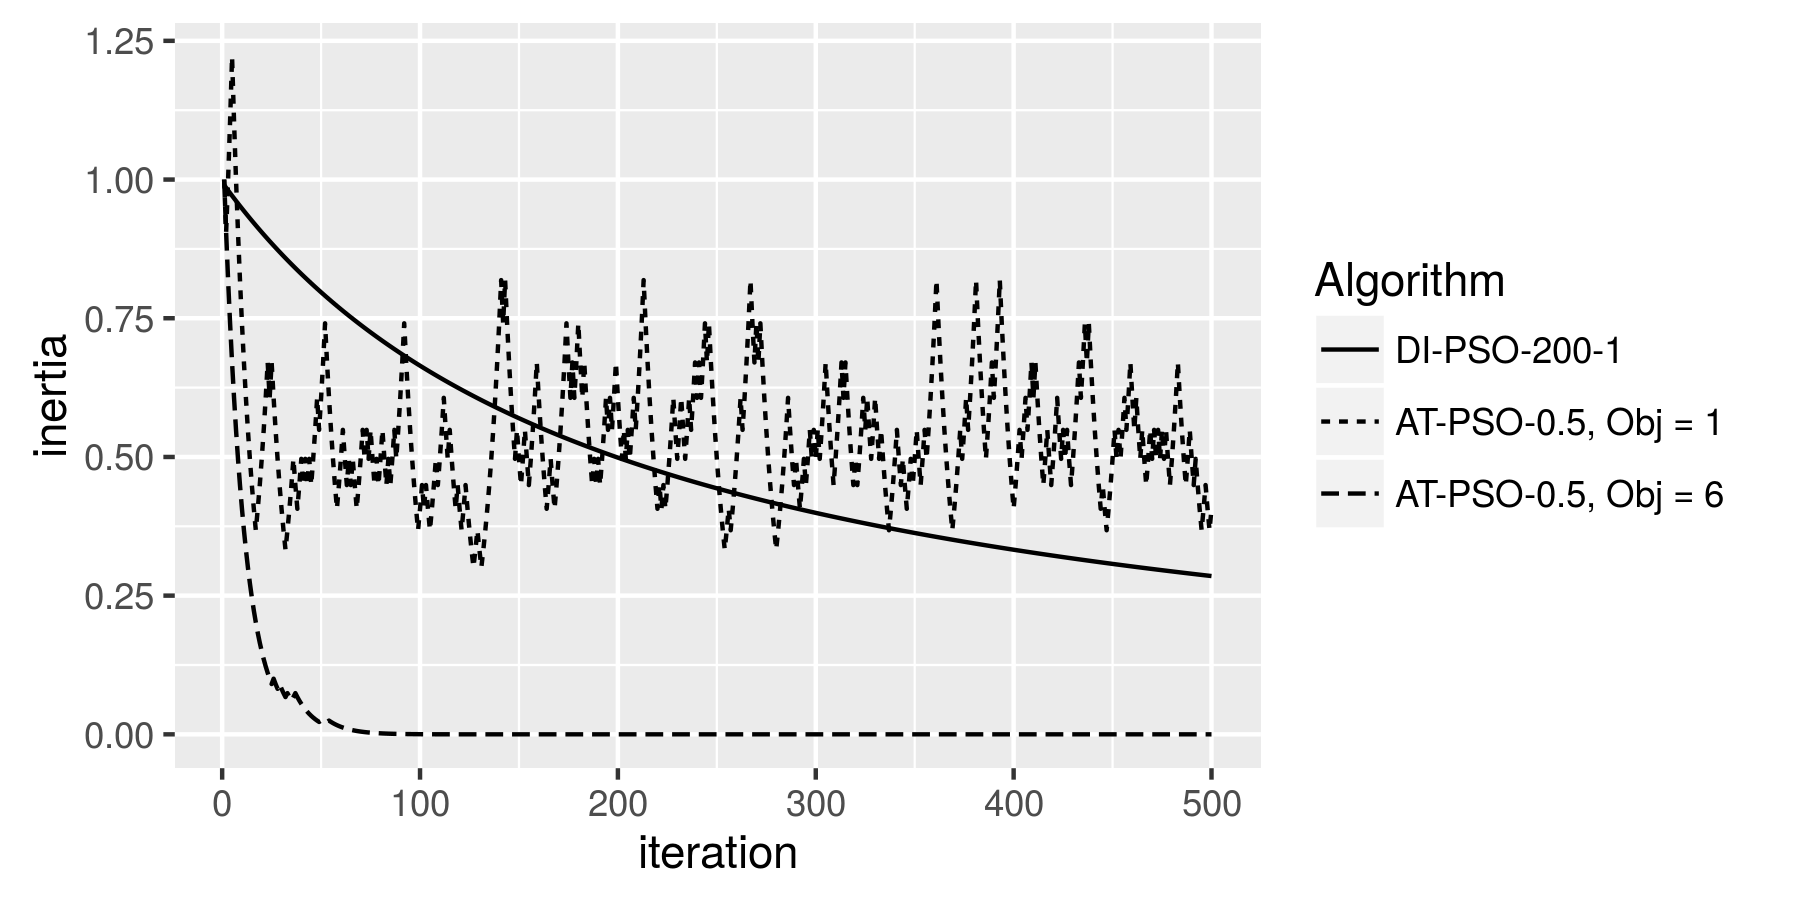
\includegraphics[width=0.95\textwidth]{psosims/inertiaplot.png}
\caption{Inertia over time for the DI-PSO algorithm with $\alpha=200$ and $\beta=1$, and for one replication of the AT-PSO-0.5 algorithm for each of OFs 1 and 6.}
\label{fig:inertia}
\end{figure}


Based on these simulations, our default recommendation is conditional. In problems where convergence is important, such as when finding the posterior mode to use for the normal approximation in a Metropolis proposal, we recommend AT-PSO with $R^*=0.3$ or $0.5$ and using a fairly restricted neighborhood (e.g., ring-1 or ring-3). These algorithms are often the best at meeting convergence criteria, especially in problems with few or no extra local optima. In difficult problems where convergence is less important (e.g., in machine learning) an AT-BBPSO variant with $df=1$ and $R^*=0.3$ or $0.5$, and again with a restrictive neighborhood seems appropriate. These sorts of algorithms seem to do a better job of getting into a region around the global max, though not as well at searching through that region. This bipartite strategy suggests a combined strategy: use AT-BBPSO or some algorithm  at first in order to quickly find a good region of the search space, then use AT-PSO to quickly search through that region. 

% latex table generated in R 3.3.1 by xtable 1.8-2 package
% Tue Jun 28 14:37:02 2016
\begin{table}[ht]
\centering
\footnotesize{
\begin{tabular}{r|rrrr|rrrr|rrrr}
\multicolumn{1}{l}{Obj = 1} & \multicolumn{4}{c}{Global nbhd} & \multicolumn{4}{c}{Ring-3 nbhd} & \multicolumn{4}{c}{Ring-1 nbhd}\\
  \hline
Algorithm & Mean & SD & $\widehat{p}_2$ & $\widehat{p}_4$ & Mean & SD & $\widehat{p}_2$ & $\widehat{p}_4$ & Mean & SD & $\widehat{p}_2$ & $\widehat{p}_4$ \\ 
  \hline
\multicolumn{1}{l|}{PSO} & 0.00 & 0.01 & 0.98 & 0.92 & 0.00 & 0.00 & 1.00 & 1.00 & 0.00 & 0.00 & 1.00 & 1.00 \\ 
  \multicolumn{1}{l|}{BBPSO-MC} & 0.12 & 0.04 & 0.00 & 0.00 & 0.09 & 0.03 & 0.00 & 0.00 & 0.04 & 0.02 & 0.06 & 0.00 \\ 
  \multicolumn{1}{l|}{BBPSOxp-MC} & 0.02 & 0.01 & 0.06 & 0.00 & 0.01 & 0.01 & 0.60 & 0.00 & 0.00 & 0.00 & 1.00 & 0.00 \\ 
\hline
\multicolumn{1}{l|}{AT-BBPSO-MC} &&&&&&&&&&&&\\
  $df = 1,\enspace$ $R^* =0.1$ & 0.02 & 0.01 & 0.02 & 0.00 & 0.01 & 0.01 & 0.22 & 0.00 & 0.00 & 0.00 & 0.96 & 0.00 \\ 
  $df = 1,\enspace$ $R^* =0.3$ & 0.02 & 0.01 & 0.06 & 0.00 & 0.01 & 0.00 & 0.22 & 0.00 & 0.00 & 0.00 & 0.96 & 0.00 \\ 
  $df = 1,\enspace$ $R^* =0.5$ & 0.02 & 0.01 & 0.04 & 0.00 & 0.01 & 0.00 & 0.10 & 0.00 & 0.00 & 0.00 & 0.96 & 0.00 \\ 
  $df = 1,\enspace$ $R^* =0.7$ & 0.02 & 0.01 & 0.06 & 0.00 & 0.01 & 0.01 & 0.22 & 0.00 & 0.00 & 0.00 & 0.98 & 0.00 \\ 
  $df = 3,\enspace$ $R^* =0.1$ & 0.04 & 0.01 & 0.02 & 0.00 & 0.03 & 0.01 & 0.00 & 0.00 & 0.01 & 0.00 & 0.70 & 0.00 \\ 
  $df = 3,\enspace$ $R^* =0.3$ & 0.04 & 0.02 & 0.00 & 0.00 & 0.03 & 0.01 & 0.00 & 0.00 & 0.01 & 0.00 & 0.56 & 0.00 \\ 
  $df = 3,\enspace$ $R^* =0.5$ & 0.04 & 0.01 & 0.00 & 0.00 & 0.03 & 0.01 & 0.02 & 0.00 & 0.01 & 0.00 & 0.60 & 0.00 \\ 
  $df = 3,\enspace$ $R^* =0.7$ & 0.04 & 0.01 & 0.00 & 0.00 & 0.03 & 0.01 & 0.02 & 0.00 & 0.01 & 0.00 & 0.64 & 0.00 \\ 
  $df = 5,\enspace$ $R^* =0.1$ & 0.06 & 0.02 & 0.00 & 0.00 & 0.04 & 0.02 & 0.00 & 0.00 & 0.01 & 0.01 & 0.32 & 0.00 \\ 
  $df = 5,\enspace$ $R^* =0.3$ & 0.06 & 0.02 & 0.00 & 0.00 & 0.04 & 0.01 & 0.00 & 0.00 & 0.02 & 0.01 & 0.26 & 0.00 \\ 
  $df = 5,\enspace$ $R^* =0.5$ & 0.06 & 0.02 & 0.00 & 0.00 & 0.04 & 0.01 & 0.00 & 0.00 & 0.01 & 0.01 & 0.34 & 0.00 \\ 
  $df = 5,\enspace$ $R^* =0.7$ & 0.06 & 0.02 & 0.00 & 0.00 & 0.04 & 0.01 & 0.00 & 0.00 & 0.01 & 0.01 & 0.36 & 0.00 \\ 
  $df = \infty,$ $R^* =0.1$ & 0.13 & 0.04 & 0.00 & 0.00 & 0.09 & 0.04 & 0.00 & 0.00 & 0.04 & 0.02 & 0.00 & 0.00 \\ 
  $df = \infty,$ $R^* =0.3$ & 0.12 & 0.04 & 0.00 & 0.00 & 0.09 & 0.02 & 0.00 & 0.00 & 0.04 & 0.02 & 0.02 & 0.00 \\ 
  $df = \infty,$ $R^* =0.5$ & 0.13 & 0.04 & 0.00 & 0.00 & 0.10 & 0.03 & 0.00 & 0.00 & 0.04 & 0.02 & 0.02 & 0.00 \\ 
  $df = \infty,$ $R^* =0.7$ & 0.12 & 0.04 & 0.00 & 0.00 & 0.09 & 0.03 & 0.00 & 0.00 & 0.03 & 0.02 & 0.00 & 0.00 \\ 
\hline
\multicolumn{1}{l|}{AT-BBPSOxp-MC} &&&&&&&&&&&&\\
  $df = 1,\enspace$ $R^* =0.1$ & 0.00 & 0.00 & 0.98 & 0.00 & 0.00 & 0.00 & 1.00 & 0.00 & 0.00 & 0.00 & 1.00 & 0.20 \\ 
  $df = 1,\enspace$ $R^* =0.3$ & 0.00 & 0.00 & 0.98 & 0.00 & 0.00 & 0.00 & 1.00 & 0.00 & 0.00 & 0.00 & 1.00 & 0.32 \\ 
  $df = 1,\enspace$ $R^* =0.5$ & 0.00 & 0.00 & 1.00 & 0.00 & 0.00 & 0.00 & 1.00 & 0.00 & 0.00 & 0.00 & 1.00 & 0.26 \\ 
  $df = 1,\enspace$ $R^* =0.7$ & 0.00 & 0.00 & 1.00 & 0.00 & 0.00 & 0.00 & 1.00 & 0.00 & 0.00 & 0.00 & 1.00 & 0.20 \\ 
  $df = 3,\enspace$ $R^* =0.1$ & 0.01 & 0.00 & 0.90 & 0.00 & 0.00 & 0.00 & 1.00 & 0.00 & 0.00 & 0.00 & 1.00 & 0.10 \\ 
  $df = 3,\enspace$ $R^* =0.3$ & 0.01 & 0.00 & 0.94 & 0.00 & 0.00 & 0.00 & 1.00 & 0.00 & 0.00 & 0.00 & 1.00 & 0.10 \\ 
  $df = 3,\enspace$ $R^* =0.5$ & 0.01 & 0.00 & 0.88 & 0.00 & 0.00 & 0.00 & 1.00 & 0.00 & 0.00 & 0.00 & 1.00 & 0.06 \\ 
  $df = 3,\enspace$ $R^* =0.7$ & 0.01 & 0.00 & 0.90 & 0.00 & 0.00 & 0.00 & 1.00 & 0.00 & 0.00 & 0.00 & 1.00 & 0.08 \\ 
  $df = 5,\enspace$ $R^* =0.1$ & 0.01 & 0.00 & 0.64 & 0.00 & 0.00 & 0.00 & 1.00 & 0.00 & 0.00 & 0.00 & 1.00 & 0.08 \\ 
  $df = 5,\enspace$ $R^* =0.3$ & 0.01 & 0.00 & 0.50 & 0.00 & 0.00 & 0.00 & 0.96 & 0.00 & 0.00 & 0.00 & 1.00 & 0.02 \\ 
  $df = 5,\enspace$ $R^* =0.5$ & 0.01 & 0.00 & 0.58 & 0.00 & 0.00 & 0.00 & 0.98 & 0.00 & 0.00 & 0.00 & 1.00 & 0.02 \\ 
  $df = 5,\enspace$ $R^* =0.7$ & 0.01 & 0.00 & 0.54 & 0.00 & 0.00 & 0.00 & 1.00 & 0.00 & 0.00 & 0.00 & 1.00 & 0.04 \\ 
  $df = \infty,$ $R^* =0.1$ & 0.02 & 0.01 & 0.00 & 0.00 & 0.01 & 0.00 & 0.58 & 0.00 & 0.00 & 0.00 & 1.00 & 0.00 \\ 
  $df = \infty,$ $R^* =0.3$ & 0.02 & 0.01 & 0.06 & 0.00 & 0.01 & 0.00 & 0.52 & 0.00 & 0.00 & 0.00 & 1.00 & 0.02 \\ 
  $df = \infty,$ $R^* =0.5$ & 0.02 & 0.01 & 0.10 & 0.00 & 0.01 & 0.01 & 0.60 & 0.00 & 0.00 & 0.00 & 1.00 & 0.00 \\ 
  $df = \infty,$ $R^* =0.7$ & 0.02 & 0.01 & 0.10 & 0.00 & 0.01 & 0.00 & 0.58 & 0.00 & 0.00 & 0.00 & 1.00 & 0.00 \\ 
\hline
\multicolumn{1}{l|}{DI-PSO} &&&&&&&&&&&&\\
  $\alpha = 50,\enspace$ $\beta =1$ & 54.28 & 103.76 & 0.00 & 0.00 & 0.02 & 0.08 & 0.88 & 0.46 & 0.00 & 0.01 & 0.98 & 0.66 \\ 
  $\alpha = 50,\enspace$ $\beta =2$ & 272.52 & 697.62 & 0.00 & 0.00 & 1.08 & 3.29 & 0.14 & 0.00 & 0.82 & 1.17 & 0.12 & 0.00 \\ 
  $\alpha = 50,\enspace$ $\beta =4$ & 883.23 & 1791.32 & 0.00 & 0.00 & 35.34 & 64.52 & 0.00 & 0.00 & 70.01 & 110.22 & 0.00 & 0.00 \\ 
  $\alpha = 100,$ $\beta =1$ & 3.10 & 7.30 & 0.16 & 0.00 & 0.00 & 0.00 & 1.00 & 0.94 & 0.00 & 0.00 & 1.00 & 1.00 \\ 
  $\alpha = 100,$ $\beta =2$ & 131.33 & 377.01 & 0.00 & 0.00 & 0.35 & 1.31 & 0.72 & 0.28 & 0.01 & 0.03 & 0.90 & 0.20 \\ 
  $\alpha = 100,$ $\beta =4$ & 380.00 & 756.97 & 0.00 & 0.00 & 21.23 & 77.39 & 0.02 & 0.00 & 8.73 & 20.23 & 0.00 & 0.00 \\ 
  $\alpha = 200,$ $\beta =1$ & 15.54 & 77.96 & 0.48 & 0.14 & 0.00 & 0.00 & 1.00 & 1.00 & 0.00 & 0.00 & 1.00 & 1.00 \\ 
  $\alpha = 200,$ $\beta =2$ & 77.09 & 233.84 & 0.10 & 0.00 & 0.00 & 0.00 & 1.00 & 0.88 & 0.00 & 0.00 & 1.00 & 1.00 \\ 
  $\alpha = 200,$ $\beta =4$ & 306.53 & 462.20 & 0.00 & 0.00 & 7.72 & 39.48 & 0.34 & 0.02 & 0.57 & 2.02 & 0.28 & 0.00 \\ 
\hline
\multicolumn{1}{l|}{AT-PSO} &&&&&&&&&&&&\\
  $R^* = 0.1$ & 0.00 & 0.00 & 1.00 & 1.00 & 0.00 & 0.00 & 1.00 & 1.00 & 6.49 & 20.38 & 0.12 & 0.00 \\ 
  $R^* = 0.3$ & 0.00 & 0.00 & 1.00 & 1.00 & 0.00 & 0.00 & 1.00 & 1.00 & 0.00 & 0.00 & 1.00 & 1.00 \\ 
  $R^* = 0.5$ & 0.00 & 0.02 & 0.98 & 0.84 & 0.00 & 0.00 & 1.00 & 1.00 & 0.00 & 0.00 & 1.00 & 1.00 \\ 
  $R^* = 0.7$ & 10.19 & 30.90 & 0.20 & 0.12 & 0.00 & 0.00 & 1.00 & 1.00 & 0.00 & 0.00 & 1.00 & 1.00 \\ 
   \hline
\end{tabular}
}
\caption{Simulation results for OF1 with $D=20$. Each PSO algorithm was initiated in a range that did not contain the true maximum with 20 particles and run for 500 iterations, repeated for 50 repetitions. The Mean and SD columns represent the mean and standard deviation of the difference between the found maximum and the true maximum, while $\widehat{p}_i$ denotes the proportion of the repetitions that ended within $10^{-i}$ of the true maximum for $i=2,4$.}
\label{tab:psosim1}
\end{table}
% latex table generated in R 3.3.1 by xtable 1.8-2 package
% Tue Jun 28 14:37:02 2016
\begin{table}[ht]
\centering
\footnotesize{
\begin{tabular}{r|rrrr|rrrr|rrrr}
\multicolumn{1}{l}{Obj = 2} & \multicolumn{4}{c}{Global nbhd} & \multicolumn{4}{c}{Ring-3 nbhd} & \multicolumn{4}{c}{Ring-1 nbhd}\\
  \hline
Algorithm & Mean & SD & $\widehat{p}_2$ & $\widehat{p}_4$ & Mean & SD & $\widehat{p}_2$ & $\widehat{p}_4$ & Mean & SD & $\widehat{p}_2$ & $\widehat{p}_4$ \\ 
  \hline
\multicolumn{1}{l|}{PSO} & 15.69 & 80.28 & 0.66 & 0.42 & 0.01 & 0.01 & 0.86 & 0.10 & 1.92 & 4.16 & 0.00 & 0.00 \\ 
  \multicolumn{1}{l|}{BBPSO-MC} & 0.43 & 0.13 & 0.00 & 0.00 & 0.47 & 0.23 & 0.00 & 0.00 & 0.72 & 0.53 & 0.00 & 0.00 \\ 
  \multicolumn{1}{l|}{BBPSOxp-MC} & 2.10 & 1.59 & 0.00 & 0.00 & 3.64 & 4.33 & 0.00 & 0.00 & 3.20 & 7.55 & 0.00 & 0.00 \\ 
\hline
\multicolumn{1}{l|}{AT-BBPSO-MC} &&&&&&&&&&&&\\
  $df = 1,\enspace$ $R^* =0.1$ & 0.17 & 0.10 & 0.00 & 0.00 & 0.18 & 0.09 & 0.00 & 0.00 & 0.10 & 0.08 & 0.00 & 0.00 \\ 
  $df = 1,\enspace$ $R^* =0.3$ & 0.19 & 0.08 & 0.00 & 0.00 & 0.17 & 0.09 & 0.00 & 0.00 & 0.10 & 0.06 & 0.00 & 0.00 \\ 
  $df = 1,\enspace$ $R^* =0.5$ & 0.17 & 0.09 & 0.00 & 0.00 & 0.19 & 0.11 & 0.00 & 0.00 & 0.16 & 0.14 & 0.00 & 0.00 \\ 
  $df = 1,\enspace$ $R^* =0.7$ & 0.18 & 0.09 & 0.00 & 0.00 & 0.16 & 0.09 & 0.00 & 0.00 & 0.11 & 0.09 & 0.00 & 0.00 \\ 
  $df = 3,\enspace$ $R^* =0.1$ & 0.20 & 0.08 & 0.00 & 0.00 & 0.18 & 0.10 & 0.00 & 0.00 & 0.17 & 0.17 & 0.00 & 0.00 \\ 
  $df = 3,\enspace$ $R^* =0.3$ & 0.20 & 0.08 & 0.00 & 0.00 & 0.18 & 0.08 & 0.00 & 0.00 & 0.12 & 0.08 & 0.00 & 0.00 \\ 
  $df = 3,\enspace$ $R^* =0.5$ & 0.20 & 0.09 & 0.00 & 0.00 & 0.19 & 0.09 & 0.00 & 0.00 & 0.12 & 0.07 & 0.00 & 0.00 \\ 
  $df = 3,\enspace$ $R^* =0.7$ & 0.21 & 0.08 & 0.00 & 0.00 & 0.22 & 0.08 & 0.00 & 0.00 & 0.12 & 0.10 & 0.00 & 0.00 \\ 
  $df = 5,\enspace$ $R^* =0.1$ & 0.26 & 0.10 & 0.00 & 0.00 & 0.22 & 0.10 & 0.00 & 0.00 & 0.16 & 0.09 & 0.00 & 0.00 \\ 
  $df = 5,\enspace$ $R^* =0.3$ & 0.27 & 0.13 & 0.00 & 0.00 & 0.24 & 0.09 & 0.00 & 0.00 & 0.17 & 0.11 & 0.00 & 0.00 \\ 
  $df = 5,\enspace$ $R^* =0.5$ & 0.25 & 0.08 & 0.00 & 0.00 & 0.24 & 0.10 & 0.00 & 0.00 & 0.16 & 0.10 & 0.00 & 0.00 \\ 
  $df = 5,\enspace$ $R^* =0.7$ & 0.27 & 0.09 & 0.00 & 0.00 & 0.20 & 0.09 & 0.00 & 0.00 & 0.19 & 0.10 & 0.00 & 0.00 \\ 
  $df = \infty,$ $R^* =0.1$ & 0.45 & 0.18 & 0.00 & 0.00 & 0.47 & 0.17 & 0.00 & 0.00 & 0.58 & 0.65 & 0.00 & 0.00 \\ 
  $df = \infty,$ $R^* =0.3$ & 0.52 & 0.22 & 0.00 & 0.00 & 0.46 & 0.20 & 0.00 & 0.00 & 0.57 & 0.38 & 0.00 & 0.00 \\ 
  $df = \infty,$ $R^* =0.5$ & 0.42 & 0.17 & 0.00 & 0.00 & 0.42 & 0.15 & 0.00 & 0.00 & 0.66 & 0.63 & 0.00 & 0.00 \\ 
  $df = \infty,$ $R^* =0.7$ & 0.45 & 0.20 & 0.00 & 0.00 & 0.46 & 0.18 & 0.00 & 0.00 & 0.60 & 0.46 & 0.00 & 0.00 \\ 
\hline
\multicolumn{1}{l|}{AT-BBPSOxp-MC} &&&&&&&&&&&&\\
  $df = 1,\enspace$ $R^* =0.1$ & 1.32 & 0.93 & 0.00 & 0.00 & 0.97 & 0.95 & 0.00 & 0.00 & 0.29 & 0.36 & 0.00 & 0.00 \\ 
  $df = 1,\enspace$ $R^* =0.3$ & 1.33 & 1.25 & 0.00 & 0.00 & 0.98 & 0.86 & 0.00 & 0.00 & 0.23 & 0.26 & 0.00 & 0.00 \\ 
  $df = 1,\enspace$ $R^* =0.5$ & 1.55 & 1.65 & 0.00 & 0.00 & 1.09 & 1.76 & 0.00 & 0.00 & 0.27 & 0.44 & 0.00 & 0.00 \\ 
  $df = 1,\enspace$ $R^* =0.7$ & 1.07 & 0.83 & 0.00 & 0.00 & 1.10 & 1.05 & 0.00 & 0.00 & 0.19 & 0.11 & 0.00 & 0.00 \\ 
  $df = 3,\enspace$ $R^* =0.1$ & 0.72 & 0.56 & 0.00 & 0.00 & 0.69 & 0.50 & 0.00 & 0.00 & 0.29 & 0.24 & 0.00 & 0.00 \\ 
  $df = 3,\enspace$ $R^* =0.3$ & 0.70 & 0.45 & 0.00 & 0.00 & 0.95 & 1.25 & 0.00 & 0.00 & 0.25 & 0.31 & 0.00 & 0.00 \\ 
  $df = 3,\enspace$ $R^* =0.5$ & 0.63 & 0.35 & 0.00 & 0.00 & 0.77 & 0.66 & 0.00 & 0.00 & 0.36 & 0.48 & 0.00 & 0.00 \\ 
  $df = 3,\enspace$ $R^* =0.7$ & 0.64 & 0.49 & 0.00 & 0.00 & 0.73 & 0.47 & 0.00 & 0.00 & 0.32 & 0.42 & 0.00 & 0.00 \\ 
  $df = 5,\enspace$ $R^* =0.1$ & 0.69 & 0.42 & 0.00 & 0.00 & 1.83 & 5.74 & 0.00 & 0.00 & 0.77 & 1.64 & 0.00 & 0.00 \\ 
  $df = 5,\enspace$ $R^* =0.3$ & 0.80 & 0.49 & 0.00 & 0.00 & 0.93 & 0.77 & 0.00 & 0.00 & 0.50 & 0.45 & 0.00 & 0.00 \\ 
  $df = 5,\enspace$ $R^* =0.5$ & 0.99 & 0.79 & 0.00 & 0.00 & 0.83 & 0.69 & 0.00 & 0.00 & 0.73 & 1.06 & 0.00 & 0.00 \\ 
  $df = 5,\enspace$ $R^* =0.7$ & 0.76 & 0.47 & 0.00 & 0.00 & 0.80 & 0.72 & 0.00 & 0.00 & 0.38 & 0.40 & 0.00 & 0.00 \\ 
  $df = \infty,$ $R^* =0.1$ & 2.05 & 1.82 & 0.00 & 0.00 & 4.80 & 6.08 & 0.00 & 0.00 & 4.89 & 8.52 & 0.00 & 0.00 \\ 
  $df = \infty,$ $R^* =0.3$ & 1.53 & 0.80 & 0.00 & 0.00 & 3.90 & 4.95 & 0.00 & 0.00 & 5.17 & 17.76 & 0.00 & 0.00 \\ 
  $df = \infty,$ $R^* =0.5$ & 2.48 & 3.39 & 0.00 & 0.00 & 5.39 & 5.48 & 0.00 & 0.00 & 6.77 & 14.34 & 0.00 & 0.00 \\ 
  $df = \infty,$ $R^* =0.7$ & 2.00 & 1.95 & 0.00 & 0.00 & 4.98 & 7.45 & 0.00 & 0.00 & 5.33 & 10.20 & 0.00 & 0.00 \\ 
\hline
\multicolumn{1}{l|}{DI-PSO} &&&&&&&&&&&&\\
  $\alpha = 50,\enspace$ $\beta =1$ & 1766.75 & 1809.97 & 0.00 & 0.00 & 312.79 & 656.97 & 0.00 & 0.00 & 247.82 & 283.72 & 0.00 & 0.00 \\ 
  $\alpha = 50,\enspace$ $\beta =2$ & 2130.86 & 1542.98 & 0.00 & 0.00 & 748.09 & 740.09 & 0.00 & 0.00 & 710.64 & 654.96 & 0.00 & 0.00 \\ 
  $\alpha = 50,\enspace$ $\beta =4$ & 4033.77 & 3078.76 & 0.00 & 0.00 & 1429.21 & 1150.46 & 0.00 & 0.00 & 1080.86 & 813.64 & 0.00 & 0.00 \\ 
  $\alpha = 100,$ $\beta =1$ & 691.51 & 844.60 & 0.00 & 0.00 & 30.60 & 44.85 & 0.00 & 0.00 & 28.75 & 37.66 & 0.00 & 0.00 \\ 
  $\alpha = 100,$ $\beta =2$ & 1268.37 & 1340.50 & 0.00 & 0.00 & 224.65 & 353.68 & 0.00 & 0.00 & 245.26 & 235.69 & 0.00 & 0.00 \\ 
  $\alpha = 100,$ $\beta =4$ & 3796.32 & 3766.60 & 0.00 & 0.00 & 965.39 & 781.49 & 0.00 & 0.00 & 815.09 & 734.56 & 0.00 & 0.00 \\ 
  $\alpha = 200,$ $\beta =1$ & 183.38 & 296.44 & 0.00 & 0.00 & 1.89 & 8.81 & 0.16 & 0.02 & 3.77 & 5.72 & 0.00 & 0.00 \\ 
  $\alpha = 200,$ $\beta =2$ & 1399.72 & 1907.35 & 0.00 & 0.00 & 46.32 & 67.92 & 0.00 & 0.00 & 62.39 & 78.82 & 0.00 & 0.00 \\ 
  $\alpha = 200,$ $\beta =4$ & 2832.28 & 2340.56 & 0.00 & 0.00 & 504.02 & 469.28 & 0.00 & 0.00 & 434.14 & 387.50 & 0.00 & 0.00 \\ 
\hline
\multicolumn{1}{l|}{AT-PSO} &&&&&&&&&&&&\\
  $R^* = 0.1$ & 0.02 & 0.11 & 0.78 & 0.14 & 0.04 & 0.09 & 0.58 & 0.00 & 272.50 & 538.58 & 0.00 & 0.00 \\ 
  $R^* = 0.3$ & 4.29 & 20.28 & 0.54 & 0.20 & 0.00 & 0.00 & 1.00 & 1.00 & 0.17 & 0.22 & 0.18 & 0.00 \\ 
  $R^* = 0.5$ & 601.56 & 898.19 & 0.00 & 0.00 & 0.00 & 0.00 & 1.00 & 0.72 & 0.20 & 0.36 & 0.16 & 0.00 \\ 
  $R^* = 0.7$ & 1649.00 & 1551.31 & 0.00 & 0.00 & 3.53 & 8.87 & 0.04 & 0.00 & 15.76 & 21.99 & 0.00 & 0.00 \\ 
   \hline
\end{tabular}
}
\caption{Simulation results for OF2 with $D=20$. Each PSO algorithm was initiated in a range that did not contain the true maximum with 20 particles and run for 500 iterations, repeated for 50 repetitions. The Mean and SD columns represent the mean and standard deviation of the difference between the found maximum and the true maximum, while $\widehat{p}_i$ denotes the proportion of the repetitions that ended within $10^{-i}$ of the true maximum for $i=2,4$.}
\label{tab:psosim2}
\end{table}
% latex table generated in R 3.3.1 by xtable 1.8-2 package
% Tue Jun 28 14:37:02 2016
\begin{table}[ht]
\centering
\footnotesize{
\begin{tabular}{r|rrrr|rrrr|rrrr}
\multicolumn{1}{l}{Obj = 3} & \multicolumn{4}{c}{Global nbhd} & \multicolumn{4}{c}{Ring-3 nbhd} & \multicolumn{4}{c}{Ring-1 nbhd}\\
  \hline
Algorithm & Mean & SD & $\widehat{p}_2$ & $\widehat{p}_4$ & Mean & SD & $\widehat{p}_2$ & $\widehat{p}_4$ & Mean & SD & $\widehat{p}_2$ & $\widehat{p}_4$ \\ 
  \hline
\multicolumn{1}{l|}{PSO} & 144.46 & 295.40 & 0.00 & 0.00 & 35.66 & 54.01 & 0.04 & 0.00 & 25.95 & 68.25 & 0.00 & 0.00 \\ 
  \multicolumn{1}{l|}{BBPSO-MC} & 131.31 & 90.51 & 0.00 & 0.00 & 110.19 & 63.02 & 0.00 & 0.00 & 84.45 & 71.65 & 0.00 & 0.00 \\ 
  \multicolumn{1}{l|}{BBPSOxp-MC} & 37.56 & 14.15 & 0.00 & 0.00 & 25.53 & 8.62 & 0.00 & 0.00 & 18.77 & 6.24 & 0.00 & 0.00 \\ 
\hline
\multicolumn{1}{l|}{AT-BBPSO-MC} &&&&&&&&&&&&\\
  $df = 1,\enspace$ $R^* =0.1$ & 111.48 & 250.62 & 0.00 & 0.00 & 53.72 & 43.43 & 0.00 & 0.00 & 110.78 & 165.53 & 0.00 & 0.00 \\ 
  $df = 1,\enspace$ $R^* =0.3$ & 149.32 & 242.67 & 0.00 & 0.00 & 90.41 & 154.44 & 0.00 & 0.00 & 60.90 & 60.45 & 0.00 & 0.00 \\ 
  $df = 1,\enspace$ $R^* =0.5$ & 106.08 & 127.98 & 0.00 & 0.00 & 78.98 & 111.62 & 0.00 & 0.00 & 49.87 & 53.05 & 0.00 & 0.00 \\ 
  $df = 1,\enspace$ $R^* =0.7$ & 120.35 & 187.50 & 0.00 & 0.00 & 79.60 & 107.68 & 0.00 & 0.00 & 83.29 & 126.26 & 0.00 & 0.00 \\ 
  $df = 3,\enspace$ $R^* =0.1$ & 114.66 & 118.03 & 0.00 & 0.00 & 88.22 & 58.20 & 0.00 & 0.00 & 69.83 & 60.08 & 0.00 & 0.00 \\ 
  $df = 3,\enspace$ $R^* =0.3$ & 144.03 & 225.00 & 0.00 & 0.00 & 78.97 & 65.90 & 0.00 & 0.00 & 73.54 & 100.15 & 0.00 & 0.00 \\ 
  $df = 3,\enspace$ $R^* =0.5$ & 121.44 & 127.02 & 0.00 & 0.00 & 79.52 & 71.45 & 0.00 & 0.00 & 57.98 & 48.82 & 0.00 & 0.00 \\ 
  $df = 3,\enspace$ $R^* =0.7$ & 108.30 & 81.33 & 0.00 & 0.00 & 71.77 & 64.65 & 0.00 & 0.00 & 54.11 & 46.59 & 0.00 & 0.00 \\ 
  $df = 5,\enspace$ $R^* =0.1$ & 125.89 & 116.43 & 0.00 & 0.00 & 78.12 & 32.51 & 0.00 & 0.00 & 71.77 & 44.25 & 0.00 & 0.00 \\ 
  $df = 5,\enspace$ $R^* =0.3$ & 108.21 & 69.88 & 0.00 & 0.00 & 94.78 & 44.39 & 0.00 & 0.00 & 67.79 & 65.60 & 0.00 & 0.00 \\ 
  $df = 5,\enspace$ $R^* =0.5$ & 111.18 & 90.71 & 0.00 & 0.00 & 78.14 & 35.93 & 0.00 & 0.00 & 68.41 & 67.38 & 0.00 & 0.00 \\ 
  $df = 5,\enspace$ $R^* =0.7$ & 107.09 & 63.45 & 0.00 & 0.00 & 93.72 & 69.07 & 0.00 & 0.00 & 71.64 & 92.09 & 0.00 & 0.00 \\ 
  $df = \infty,$ $R^* =0.1$ & 126.16 & 71.55 & 0.00 & 0.00 & 99.98 & 25.30 & 0.00 & 0.00 & 68.42 & 43.53 & 0.00 & 0.00 \\ 
  $df = \infty,$ $R^* =0.3$ & 127.38 & 66.15 & 0.00 & 0.00 & 103.96 & 31.69 & 0.00 & 0.00 & 68.21 & 54.76 & 0.00 & 0.00 \\ 
  $df = \infty,$ $R^* =0.5$ & 109.58 & 30.42 & 0.00 & 0.00 & 102.75 & 39.42 & 0.00 & 0.00 & 76.03 & 59.73 & 0.00 & 0.00 \\ 
  $df = \infty,$ $R^* =0.7$ & 112.31 & 31.53 & 0.00 & 0.00 & 111.33 & 47.31 & 0.00 & 0.00 & 72.48 & 29.60 & 0.00 & 0.00 \\ 
\hline
\multicolumn{1}{l|}{AT-BBPSOxp-MC} &&&&&&&&&&&&\\
  $df = 1,\enspace$ $R^* =0.1$ & 54.91 & 71.36 & 0.00 & 0.00 & 46.43 & 53.25 & 0.00 & 0.00 & 27.74 & 33.78 & 0.00 & 0.00 \\ 
  $df = 1,\enspace$ $R^* =0.3$ & 42.75 & 27.54 & 0.00 & 0.00 & 34.70 & 44.52 & 0.00 & 0.00 & 26.56 & 35.25 & 0.00 & 0.00 \\ 
  $df = 1,\enspace$ $R^* =0.5$ & 47.05 & 33.70 & 0.00 & 0.00 & 52.38 & 84.94 & 0.00 & 0.00 & 35.21 & 47.68 & 0.00 & 0.00 \\ 
  $df = 1,\enspace$ $R^* =0.7$ & 44.34 & 44.22 & 0.00 & 0.00 & 55.48 & 108.75 & 0.00 & 0.00 & 39.44 & 46.50 & 0.00 & 0.00 \\ 
  $df = 3,\enspace$ $R^* =0.1$ & 34.88 & 12.52 & 0.00 & 0.00 & 35.55 & 22.20 & 0.00 & 0.00 & 19.04 & 13.27 & 0.00 & 0.00 \\ 
  $df = 3,\enspace$ $R^* =0.3$ & 40.08 & 14.57 & 0.00 & 0.00 & 33.62 & 25.98 & 0.00 & 0.00 & 23.77 & 19.44 & 0.00 & 0.00 \\ 
  $df = 3,\enspace$ $R^* =0.5$ & 44.76 & 48.60 & 0.00 & 0.00 & 27.92 & 12.79 & 0.00 & 0.00 & 27.27 & 35.43 & 0.00 & 0.00 \\ 
  $df = 3,\enspace$ $R^* =0.7$ & 46.32 & 77.32 & 0.00 & 0.00 & 30.46 & 14.12 & 0.00 & 0.00 & 18.80 & 8.33 & 0.00 & 0.00 \\ 
  $df = 5,\enspace$ $R^* =0.1$ & 40.72 & 15.41 & 0.00 & 0.00 & 35.09 & 28.26 & 0.00 & 0.00 & 20.00 & 19.18 & 0.00 & 0.00 \\ 
  $df = 5,\enspace$ $R^* =0.3$ & 40.81 & 22.60 & 0.00 & 0.00 & 32.33 & 19.05 & 0.00 & 0.00 & 20.36 & 12.27 & 0.00 & 0.00 \\ 
  $df = 5,\enspace$ $R^* =0.5$ & 43.59 & 51.50 & 0.00 & 0.00 & 43.91 & 76.14 & 0.00 & 0.00 & 29.54 & 51.03 & 0.00 & 0.00 \\ 
  $df = 5,\enspace$ $R^* =0.7$ & 38.25 & 13.76 & 0.00 & 0.00 & 29.31 & 12.40 & 0.00 & 0.00 & 21.43 & 26.09 & 0.00 & 0.00 \\ 
  $df = \infty,$ $R^* =0.1$ & 40.62 & 19.73 & 0.00 & 0.00 & 31.86 & 18.35 & 0.00 & 0.00 & 25.61 & 42.18 & 0.00 & 0.00 \\ 
  $df = \infty,$ $R^* =0.3$ & 37.54 & 31.58 & 0.00 & 0.00 & 27.73 & 9.34 & 0.00 & 0.00 & 17.79 & 6.45 & 0.00 & 0.00 \\ 
  $df = \infty,$ $R^* =0.5$ & 39.05 & 14.07 & 0.00 & 0.00 & 27.79 & 8.39 & 0.00 & 0.00 & 20.38 & 6.64 & 0.00 & 0.00 \\ 
  $df = \infty,$ $R^* =0.7$ & 35.58 & 12.57 & 0.00 & 0.00 & 28.22 & 8.33 & 0.00 & 0.00 & 18.96 & 7.86 & 0.00 & 0.00 \\ 
\hline
\multicolumn{1}{l|}{DI-PSO} &&&&&&&&&&&&\\
  $\alpha = 50,\enspace$ $\beta =1$ & 1349.13 & 1940.53 & 0.00 & 0.00 & 200.09 & 245.80 & 0.00 & 0.00 & 149.74 & 221.74 & 0.00 & 0.00 \\ 
  $\alpha = 50,\enspace$ $\beta =2$ & 7204.93 & 16333.63 & 0.00 & 0.00 & 785.95 & 2896.36 & 0.00 & 0.00 & 339.44 & 446.58 & 0.00 & 0.00 \\ 
  $\alpha = 50,\enspace$ $\beta =4$ & 24307.11 & 42723.81 & 0.00 & 0.00 & 7881.86 & 26566.77 & 0.00 & 0.00 & 19136.28 & 43990.37 & 0.00 & 0.00 \\ 
  $\alpha = 100,$ $\beta =1$ & 420.14 & 827.79 & 0.00 & 0.00 & 108.58 & 211.14 & 0.00 & 0.00 & 78.35 & 107.85 & 0.00 & 0.00 \\ 
  $\alpha = 100,$ $\beta =2$ & 1245.63 & 1717.55 & 0.00 & 0.00 & 653.55 & 2182.72 & 0.00 & 0.00 & 214.47 & 545.19 & 0.00 & 0.00 \\ 
  $\alpha = 100,$ $\beta =4$ & 33664.67 & 97150.26 & 0.00 & 0.00 & 1398.23 & 2729.87 & 0.00 & 0.00 & 2100.05 & 4701.80 & 0.00 & 0.00 \\ 
  $\alpha = 200,$ $\beta =1$ & 636.50 & 1081.78 & 0.00 & 0.00 & 101.35 & 197.94 & 0.00 & 0.00 & 52.42 & 71.41 & 0.02 & 0.00 \\ 
  $\alpha = 200,$ $\beta =2$ & 1013.55 & 2221.85 & 0.00 & 0.00 & 237.69 & 524.60 & 0.00 & 0.00 & 144.29 & 270.95 & 0.00 & 0.00 \\ 
  $\alpha = 200,$ $\beta =4$ & 12140.28 & 30312.75 & 0.00 & 0.00 & 3804.18 & 20640.37 & 0.00 & 0.00 & 1031.02 & 2712.71 & 0.00 & 0.00 \\ 
\hline
\multicolumn{1}{l|}{AT-PSO} &&&&&&&&&&&&\\
  $R^* = 0.1$ & 76.28 & 161.98 & 0.00 & 0.00 & 92.06 & 184.12 & 0.00 & 0.00 & 3963.70 & 12776.53 & 0.00 & 0.00 \\ 
  $R^* = 0.3$ & 132.79 & 162.86 & 0.00 & 0.00 & 50.07 & 101.57 & 0.00 & 0.00 & 61.91 & 139.04 & 0.00 & 0.00 \\ 
  $R^* = 0.5$ & 239.14 & 413.19 & 0.00 & 0.00 & 79.24 & 139.68 & 0.00 & 0.00 & 48.67 & 81.20 & 0.02 & 0.02 \\ 
  $R^* = 0.7$ & 673.23 & 1512.39 & 0.00 & 0.00 & 86.14 & 193.93 & 0.00 & 0.00 & 90.40 & 117.98 & 0.00 & 0.00 \\ 
   \hline
\end{tabular}
}
\caption{Simulation results for OF3 with $D=20$. Each PSO algorithm was initiated in a range that did not contain the true maximum with 20 particles and run for 500 iterations, repeated for 50 repetitions. The Mean and SD columns represent the mean and standard deviation of the difference between the found maximum and the true maximum, while $\widehat{p}_i$ denotes the proportion of the repetitions that ended within $10^{-i}$ of the true maximum for $i=2,4$.}
\label{tab:psosim3}
\end{table}
% latex table generated in R 3.3.1 by xtable 1.8-2 package
% Tue Jun 28 14:37:02 2016
\begin{table}[ht]
\centering
\footnotesize{
\begin{tabular}{r|rrrr|rrrr|rrrr}
\multicolumn{1}{l}{Obj = 4} & \multicolumn{4}{c}{Global nbhd} & \multicolumn{4}{c}{Ring-3 nbhd} & \multicolumn{4}{c}{Ring-1 nbhd}\\
  \hline
Algorithm & Mean & SD & $\widehat{p}_2$ & $\widehat{p}_4$ & Mean & SD & $\widehat{p}_2$ & $\widehat{p}_4$ & Mean & SD & $\widehat{p}_2$ & $\widehat{p}_4$ \\ 
  \hline
\multicolumn{1}{l|}{PSO} & 4.32 & 2.75 & 0.02 & 0.02 & 0.65 & 0.89 & 0.56 & 0.56 & 0.13 & 0.47 & 0.90 & 0.86 \\ 
  \multicolumn{1}{l|}{BBPSO-MC} & 2.75 & 0.93 & 0.00 & 0.00 & 2.67 & 0.81 & 0.00 & 0.00 & 1.47 & 1.00 & 0.00 & 0.00 \\ 
  \multicolumn{1}{l|}{BBPSOxp-MC} & 0.13 & 0.05 & 0.00 & 0.00 & 0.04 & 0.02 & 0.04 & 0.00 & 0.01 & 0.00 & 0.86 & 0.00 \\ 
\hline
\multicolumn{1}{l|}{AT-BBPSO-MC} &&&&&&&&&&&&\\
  $df = 1,\enspace$ $R^* =0.1$ & 1.02 & 0.80 & 0.00 & 0.00 & 0.48 & 0.38 & 0.00 & 0.00 & 0.21 & 0.23 & 0.00 & 0.00 \\ 
  $df = 1,\enspace$ $R^* =0.3$ & 1.10 & 0.88 & 0.00 & 0.00 & 0.58 & 0.39 & 0.00 & 0.00 & 0.23 & 0.28 & 0.00 & 0.00 \\ 
  $df = 1,\enspace$ $R^* =0.5$ & 0.90 & 0.66 & 0.00 & 0.00 & 0.51 & 0.33 & 0.00 & 0.00 & 0.37 & 0.42 & 0.00 & 0.00 \\ 
  $df = 1,\enspace$ $R^* =0.7$ & 0.98 & 0.68 & 0.00 & 0.00 & 0.50 & 0.31 & 0.00 & 0.00 & 0.29 & 0.43 & 0.00 & 0.00 \\ 
  $df = 3,\enspace$ $R^* =0.1$ & 1.13 & 0.56 & 0.00 & 0.00 & 0.91 & 0.42 & 0.00 & 0.00 & 0.47 & 0.48 & 0.00 & 0.00 \\ 
  $df = 3,\enspace$ $R^* =0.3$ & 1.25 & 0.54 & 0.00 & 0.00 & 0.89 & 0.52 & 0.00 & 0.00 & 0.46 & 0.48 & 0.00 & 0.00 \\ 
  $df = 3,\enspace$ $R^* =0.5$ & 1.23 & 0.48 & 0.00 & 0.00 & 0.97 & 0.48 & 0.00 & 0.00 & 0.40 & 0.47 & 0.00 & 0.00 \\ 
  $df = 3,\enspace$ $R^* =0.7$ & 1.25 & 0.63 & 0.00 & 0.00 & 1.05 & 0.64 & 0.00 & 0.00 & 0.40 & 0.45 & 0.00 & 0.00 \\ 
  $df = 5,\enspace$ $R^* =0.1$ & 1.54 & 0.64 & 0.00 & 0.00 & 1.25 & 0.53 & 0.00 & 0.00 & 0.81 & 0.62 & 0.00 & 0.00 \\ 
  $df = 5,\enspace$ $R^* =0.3$ & 1.64 & 0.48 & 0.00 & 0.00 & 1.38 & 0.63 & 0.00 & 0.00 & 0.53 & 0.49 & 0.00 & 0.00 \\ 
  $df = 5,\enspace$ $R^* =0.5$ & 1.72 & 0.60 & 0.00 & 0.00 & 1.59 & 0.77 & 0.00 & 0.00 & 0.55 & 0.47 & 0.00 & 0.00 \\ 
  $df = 5,\enspace$ $R^* =0.7$ & 1.77 & 0.66 & 0.00 & 0.00 & 1.30 & 0.67 & 0.00 & 0.00 & 0.53 & 0.43 & 0.00 & 0.00 \\ 
  $df = \infty,$ $R^* =0.1$ & 2.63 & 0.78 & 0.00 & 0.00 & 2.42 & 0.86 & 0.00 & 0.00 & 1.38 & 0.86 & 0.00 & 0.00 \\ 
  $df = \infty,$ $R^* =0.3$ & 2.52 & 0.63 & 0.00 & 0.00 & 2.51 & 0.58 & 0.00 & 0.00 & 1.22 & 0.76 & 0.00 & 0.00 \\ 
  $df = \infty,$ $R^* =0.5$ & 2.50 & 0.84 & 0.00 & 0.00 & 2.40 & 0.77 & 0.00 & 0.00 & 1.49 & 0.90 & 0.00 & 0.00 \\ 
  $df = \infty,$ $R^* =0.7$ & 2.63 & 0.66 & 0.00 & 0.00 & 2.62 & 0.72 & 0.00 & 0.00 & 1.34 & 0.95 & 0.00 & 0.00 \\ 
\hline
\multicolumn{1}{l|}{AT-BBPSOxp-MC} &&&&&&&&&&&&\\
  $df = 1,\enspace$ $R^* =0.1$ & 0.09 & 0.04 & 0.00 & 0.00 & 0.02 & 0.01 & 0.06 & 0.00 & 0.00 & 0.00 & 1.00 & 0.00 \\ 
  $df = 1,\enspace$ $R^* =0.3$ & 0.08 & 0.04 & 0.00 & 0.00 & 0.03 & 0.01 & 0.02 & 0.00 & 0.00 & 0.00 & 0.94 & 0.00 \\ 
  $df = 1,\enspace$ $R^* =0.5$ & 0.07 & 0.03 & 0.00 & 0.00 & 0.03 & 0.01 & 0.10 & 0.00 & 0.00 & 0.00 & 0.94 & 0.00 \\ 
  $df = 1,\enspace$ $R^* =0.7$ & 0.07 & 0.03 & 0.00 & 0.00 & 0.03 & 0.01 & 0.04 & 0.00 & 0.00 & 0.00 & 1.00 & 0.00 \\ 
  $df = 3,\enspace$ $R^* =0.1$ & 0.10 & 0.04 & 0.00 & 0.00 & 0.03 & 0.01 & 0.02 & 0.00 & 0.00 & 0.00 & 0.98 & 0.00 \\ 
  $df = 3,\enspace$ $R^* =0.3$ & 0.10 & 0.04 & 0.00 & 0.00 & 0.03 & 0.01 & 0.02 & 0.00 & 0.00 & 0.00 & 0.98 & 0.00 \\ 
  $df = 3,\enspace$ $R^* =0.5$ & 0.10 & 0.04 & 0.00 & 0.00 & 0.03 & 0.01 & 0.00 & 0.00 & 0.00 & 0.00 & 1.00 & 0.00 \\ 
  $df = 3,\enspace$ $R^* =0.7$ & 0.09 & 0.04 & 0.00 & 0.00 & 0.03 & 0.02 & 0.06 & 0.00 & 0.00 & 0.00 & 0.96 & 0.00 \\ 
  $df = 5,\enspace$ $R^* =0.1$ & 0.11 & 0.04 & 0.00 & 0.00 & 0.03 & 0.02 & 0.02 & 0.00 & 0.00 & 0.00 & 0.90 & 0.00 \\ 
  $df = 5,\enspace$ $R^* =0.3$ & 0.10 & 0.04 & 0.00 & 0.00 & 0.03 & 0.01 & 0.00 & 0.00 & 0.00 & 0.00 & 0.96 & 0.00 \\ 
  $df = 5,\enspace$ $R^* =0.5$ & 0.11 & 0.05 & 0.00 & 0.00 & 0.03 & 0.01 & 0.00 & 0.00 & 0.00 & 0.00 & 0.98 & 0.00 \\ 
  $df = 5,\enspace$ $R^* =0.7$ & 0.10 & 0.04 & 0.00 & 0.00 & 0.03 & 0.02 & 0.02 & 0.00 & 0.00 & 0.00 & 0.94 & 0.00 \\ 
  $df = \infty,$ $R^* =0.1$ & 0.12 & 0.05 & 0.00 & 0.00 & 0.04 & 0.02 & 0.00 & 0.00 & 0.00 & 0.00 & 0.98 & 0.02 \\ 
  $df = \infty,$ $R^* =0.3$ & 0.12 & 0.05 & 0.00 & 0.00 & 0.04 & 0.02 & 0.00 & 0.00 & 0.01 & 0.00 & 0.84 & 0.00 \\ 
  $df = \infty,$ $R^* =0.5$ & 0.13 & 0.05 & 0.00 & 0.00 & 0.04 & 0.02 & 0.00 & 0.00 & 0.01 & 0.00 & 0.86 & 0.00 \\ 
  $df = \infty,$ $R^* =0.7$ & 0.12 & 0.04 & 0.00 & 0.00 & 0.04 & 0.02 & 0.00 & 0.00 & 0.00 & 0.00 & 0.94 & 0.00 \\ 
\hline
\multicolumn{1}{l|}{DI-PSO} &&&&&&&&&&&&\\
  $\alpha = 50,\enspace$ $\beta =1$ & 4.42 & 2.42 & 0.00 & 0.00 & 1.35 & 1.07 & 0.24 & 0.12 & 0.63 & 0.89 & 0.50 & 0.26 \\ 
  $\alpha = 50,\enspace$ $\beta =2$ & 4.31 & 2.95 & 0.00 & 0.00 & 1.79 & 1.31 & 0.02 & 0.00 & 0.83 & 0.85 & 0.20 & 0.02 \\ 
  $\alpha = 50,\enspace$ $\beta =4$ & 5.98 & 3.60 & 0.00 & 0.00 & 2.38 & 1.56 & 0.00 & 0.00 & 1.49 & 1.41 & 0.04 & 0.00 \\ 
  $\alpha = 100,$ $\beta =1$ & 2.57 & 2.02 & 0.02 & 0.00 & 1.08 & 1.07 & 0.32 & 0.26 & 0.32 & 0.49 & 0.68 & 0.68 \\ 
  $\alpha = 100,$ $\beta =2$ & 4.15 & 2.84 & 0.00 & 0.00 & 1.63 & 1.26 & 0.16 & 0.04 & 0.43 & 0.90 & 0.56 & 0.14 \\ 
  $\alpha = 100,$ $\beta =4$ & 5.21 & 3.46 & 0.00 & 0.00 & 2.12 & 1.67 & 0.00 & 0.00 & 1.16 & 1.19 & 0.08 & 0.00 \\ 
  $\alpha = 200,$ $\beta =1$ & 1.51 & 1.04 & 0.16 & 0.08 & 0.93 & 0.78 & 0.30 & 0.30 & 0.29 & 0.73 & 0.80 & 0.78 \\ 
  $\alpha = 200,$ $\beta =2$ & 4.21 & 3.29 & 0.02 & 0.00 & 1.29 & 0.88 & 0.12 & 0.12 & 0.46 & 0.62 & 0.60 & 0.48 \\ 
  $\alpha = 200,$ $\beta =4$ & 4.73 & 3.22 & 0.00 & 0.00 & 1.91 & 1.45 & 0.10 & 0.00 & 0.95 & 1.04 & 0.30 & 0.00 \\ 
\hline
\multicolumn{1}{l|}{AT-PSO} &&&&&&&&&&&&\\
  $R^* = 0.1$ & 1.60 & 1.27 & 0.18 & 0.16 & 0.30 & 0.49 & 0.70 & 0.70 & 0.39 & 0.74 & 0.30 & 0.06 \\ 
  $R^* = 0.3$ & 3.80 & 2.65 & 0.02 & 0.02 & 1.18 & 1.15 & 0.38 & 0.38 & 0.27 & 0.43 & 0.72 & 0.72 \\ 
  $R^* = 0.5$ & 6.15 & 4.25 & 0.00 & 0.00 & 2.42 & 2.62 & 0.08 & 0.08 & 1.01 & 1.16 & 0.34 & 0.34 \\ 
  $R^* = 0.7$ & 7.73 & 5.24 & 0.00 & 0.00 & 3.02 & 2.12 & 0.08 & 0.08 & 3.48 & 3.53 & 0.04 & 0.04 \\ 
   \hline
\end{tabular}
}
\caption{Simulation results for OF4 with $D=20$. Each PSO algorithm was initiated in a range that did not contain the true maximum with 20 particles and run for 500 iterations, repeated for 50 repetitions. The Mean and SD columns represent the mean and standard deviation of the difference between the found maximum and the true maximum, while $\widehat{p}_i$ denotes the proportion of the repetitions that ended within $10^{-i}$ of the true maximum for $i=2,4$.}
\label{tab:psosim4}
\end{table}
% latex table generated in R 3.3.1 by xtable 1.8-2 package
% Tue Jun 28 14:37:02 2016
\begin{table}[ht]
\centering
\footnotesize{
\begin{tabular}{r|rrrr|rrrr|rrrr}
\multicolumn{1}{l}{Obj = 5} & \multicolumn{4}{c}{Global nbhd} & \multicolumn{4}{c}{Ring-3 nbhd} & \multicolumn{4}{c}{Ring-1 nbhd}\\
  \hline
Algorithm & Mean & SD & $\widehat{p}_2$ & $\widehat{p}_4$ & Mean & SD & $\widehat{p}_2$ & $\widehat{p}_4$ & Mean & SD & $\widehat{p}_2$ & $\widehat{p}_4$ \\ 
  \hline
\multicolumn{1}{l|}{PSO} & 0.18 & 0.17 & 0.00 & 0.00 & 0.07 & 0.04 & 0.06 & 0.02 & 0.06 & 0.04 & 0.04 & 0.02 \\ 
  \multicolumn{1}{l|}{BBPSO-MC} & 107.55 & 12.45 & 0.00 & 0.00 & 123.72 & 13.02 & 0.00 & 0.00 & 139.39 & 20.19 & 0.00 & 0.00 \\ 
  \multicolumn{1}{l|}{BBPSOxp-MC} & 161.19 & 16.06 & 0.00 & 0.00 & 147.39 & 15.95 & 0.00 & 0.00 & 88.54 & 22.99 & 0.00 & 0.00 \\ 
\hline
\multicolumn{1}{l|}{AT-BBPSO-MC} &&&&&&&&&&&&\\
  $df = 1,\enspace$ $R^* =0.1$ & 0.24 & 0.20 & 0.00 & 0.00 & 0.11 & 0.06 & 0.00 & 0.00 & 0.10 & 0.06 & 0.00 & 0.00 \\ 
  $df = 1,\enspace$ $R^* =0.3$ & 0.22 & 0.15 & 0.00 & 0.00 & 0.14 & 0.08 & 0.00 & 0.00 & 0.10 & 0.08 & 0.02 & 0.00 \\ 
  $df = 1,\enspace$ $R^* =0.5$ & 0.23 & 0.14 & 0.00 & 0.00 & 0.12 & 0.09 & 0.00 & 0.00 & 0.10 & 0.05 & 0.00 & 0.00 \\ 
  $df = 1,\enspace$ $R^* =0.7$ & 0.24 & 0.16 & 0.00 & 0.00 & 0.13 & 0.09 & 0.00 & 0.00 & 0.09 & 0.05 & 0.00 & 0.00 \\ 
  $df = 3,\enspace$ $R^* =0.1$ & 0.75 & 0.61 & 0.00 & 0.00 & 0.29 & 0.18 & 0.00 & 0.00 & 0.50 & 0.34 & 0.00 & 0.00 \\ 
  $df = 3,\enspace$ $R^* =0.3$ & 0.78 & 0.59 & 0.00 & 0.00 & 0.26 & 0.15 & 0.00 & 0.00 & 0.61 & 0.37 & 0.00 & 0.00 \\ 
  $df = 3,\enspace$ $R^* =0.5$ & 0.59 & 0.41 & 0.00 & 0.00 & 0.27 & 0.17 & 0.00 & 0.00 & 0.51 & 0.31 & 0.00 & 0.00 \\ 
  $df = 3,\enspace$ $R^* =0.7$ & 0.64 & 0.45 & 0.00 & 0.00 & 0.28 & 0.15 & 0.00 & 0.00 & 0.57 & 0.40 & 0.00 & 0.00 \\ 
  $df = 5,\enspace$ $R^* =0.1$ & 7.13 & 3.33 & 0.00 & 0.00 & 16.46 & 5.52 & 0.00 & 0.00 & 33.67 & 9.42 & 0.00 & 0.00 \\ 
  $df = 5,\enspace$ $R^* =0.3$ & 8.03 & 3.84 & 0.00 & 0.00 & 16.27 & 4.90 & 0.00 & 0.00 & 31.74 & 9.31 & 0.00 & 0.00 \\ 
  $df = 5,\enspace$ $R^* =0.5$ & 7.18 & 4.05 & 0.00 & 0.00 & 16.78 & 5.88 & 0.00 & 0.00 & 36.30 & 12.42 & 0.00 & 0.00 \\ 
  $df = 5,\enspace$ $R^* =0.7$ & 7.62 & 3.58 & 0.00 & 0.00 & 15.76 & 5.55 & 0.00 & 0.00 & 32.13 & 9.37 & 0.00 & 0.00 \\ 
  $df = \infty,$ $R^* =0.1$ & 108.04 & 13.07 & 0.00 & 0.00 & 122.56 & 10.67 & 0.00 & 0.00 & 138.20 & 17.14 & 0.00 & 0.00 \\ 
  $df = \infty,$ $R^* =0.3$ & 109.07 & 12.30 & 0.00 & 0.00 & 123.46 & 10.82 & 0.00 & 0.00 & 137.72 & 19.34 & 0.00 & 0.00 \\ 
  $df = \infty,$ $R^* =0.5$ & 108.41 & 13.09 & 0.00 & 0.00 & 124.54 & 11.65 & 0.00 & 0.00 & 137.44 & 19.45 & 0.00 & 0.00 \\ 
  $df = \infty,$ $R^* =0.7$ & 108.26 & 12.55 & 0.00 & 0.00 & 125.60 & 10.86 & 0.00 & 0.00 & 138.92 & 19.62 & 0.00 & 0.00 \\ 
\hline
\multicolumn{1}{l|}{AT-BBPSOxp-MC} &&&&&&&&&&&&\\
  $df = 1,\enspace$ $R^* =0.1$ & 0.09 & 0.04 & 0.00 & 0.00 & 0.08 & 0.04 & 0.00 & 0.00 & 0.05 & 0.04 & 0.02 & 0.00 \\ 
  $df = 1,\enspace$ $R^* =0.3$ & 0.10 & 0.05 & 0.00 & 0.00 & 0.08 & 0.05 & 0.06 & 0.00 & 0.06 & 0.03 & 0.02 & 0.00 \\ 
  $df = 1,\enspace$ $R^* =0.5$ & 0.10 & 0.06 & 0.00 & 0.00 & 0.08 & 0.05 & 0.00 & 0.00 & 0.07 & 0.03 & 0.02 & 0.00 \\ 
  $df = 1,\enspace$ $R^* =0.7$ & 0.10 & 0.06 & 0.00 & 0.00 & 0.08 & 0.05 & 0.00 & 0.00 & 0.06 & 0.04 & 0.06 & 0.00 \\ 
  $df = 3,\enspace$ $R^* =0.1$ & 3.37 & 2.43 & 0.00 & 0.00 & 4.40 & 2.86 & 0.00 & 0.00 & 0.90 & 0.87 & 0.00 & 0.00 \\ 
  $df = 3,\enspace$ $R^* =0.3$ & 3.18 & 2.42 & 0.00 & 0.00 & 3.26 & 1.80 & 0.00 & 0.00 & 1.10 & 1.16 & 0.00 & 0.00 \\ 
  $df = 3,\enspace$ $R^* =0.5$ & 3.27 & 2.30 & 0.00 & 0.00 & 3.59 & 3.42 & 0.00 & 0.00 & 0.97 & 1.20 & 0.00 & 0.00 \\ 
  $df = 3,\enspace$ $R^* =0.7$ & 3.71 & 2.43 & 0.00 & 0.00 & 4.97 & 4.03 & 0.00 & 0.00 & 0.83 & 0.70 & 0.00 & 0.00 \\ 
  $df = 5,\enspace$ $R^* =0.1$ & 64.33 & 10.31 & 0.00 & 0.00 & 62.16 & 10.89 & 0.00 & 0.00 & 25.49 & 10.74 & 0.00 & 0.00 \\ 
  $df = 5,\enspace$ $R^* =0.3$ & 63.62 & 10.26 & 0.00 & 0.00 & 61.79 & 12.09 & 0.00 & 0.00 & 26.34 & 10.67 & 0.00 & 0.00 \\ 
  $df = 5,\enspace$ $R^* =0.5$ & 62.01 & 10.94 & 0.00 & 0.00 & 62.58 & 9.87 & 0.00 & 0.00 & 26.15 & 13.04 & 0.00 & 0.00 \\ 
  $df = 5,\enspace$ $R^* =0.7$ & 64.75 & 10.55 & 0.00 & 0.00 & 62.63 & 11.46 & 0.00 & 0.00 & 25.45 & 10.98 & 0.00 & 0.00 \\ 
  $df = \infty,$ $R^* =0.1$ & 157.62 & 14.20 & 0.00 & 0.00 & 148.31 & 13.62 & 0.00 & 0.00 & 87.94 & 24.29 & 0.00 & 0.00 \\ 
  $df = \infty,$ $R^* =0.3$ & 160.30 & 15.23 & 0.00 & 0.00 & 146.65 & 16.52 & 0.00 & 0.00 & 87.96 & 23.07 & 0.00 & 0.00 \\ 
  $df = \infty,$ $R^* =0.5$ & 158.78 & 16.14 & 0.00 & 0.00 & 150.94 & 14.95 & 0.00 & 0.00 & 91.44 & 21.82 & 0.00 & 0.00 \\ 
  $df = \infty,$ $R^* =0.7$ & 162.49 & 16.45 & 0.00 & 0.00 & 145.00 & 16.78 & 0.00 & 0.00 & 87.56 & 20.07 & 0.00 & 0.00 \\ 
\hline
\multicolumn{1}{l|}{DI-PSO} &&&&&&&&&&&&\\
  $\alpha = 50,\enspace$ $\beta =1$ & 1.68 & 3.09 & 0.00 & 0.00 & 0.11 & 0.06 & 0.00 & 0.00 & 0.15 & 0.10 & 0.00 & 0.00 \\ 
  $\alpha = 50,\enspace$ $\beta =2$ & 1.69 & 4.30 & 0.00 & 0.00 & 0.27 & 0.33 & 0.00 & 0.00 & 0.25 & 0.13 & 0.00 & 0.00 \\ 
  $\alpha = 50,\enspace$ $\beta =4$ & 5.70 & 6.13 & 0.00 & 0.00 & 0.79 & 0.95 & 0.00 & 0.00 & 1.01 & 1.23 & 0.00 & 0.00 \\ 
  $\alpha = 100,$ $\beta =1$ & 0.53 & 1.14 & 0.00 & 0.00 & 0.08 & 0.07 & 0.06 & 0.02 & 0.09 & 0.05 & 0.00 & 0.00 \\ 
  $\alpha = 100,$ $\beta =2$ & 2.31 & 4.78 & 0.00 & 0.00 & 0.12 & 0.06 & 0.00 & 0.00 & 0.19 & 0.12 & 0.00 & 0.00 \\ 
  $\alpha = 100,$ $\beta =4$ & 5.42 & 5.89 & 0.00 & 0.00 & 0.39 & 0.39 & 0.00 & 0.00 & 0.40 & 0.27 & 0.00 & 0.00 \\ 
  $\alpha = 200,$ $\beta =1$ & 0.18 & 0.17 & 0.02 & 0.00 & 0.09 & 0.06 & 0.00 & 0.00 & 0.09 & 0.04 & 0.00 & 0.00 \\ 
  $\alpha = 200,$ $\beta =2$ & 0.78 & 1.52 & 0.00 & 0.00 & 0.10 & 0.07 & 0.00 & 0.00 & 0.12 & 0.09 & 0.00 & 0.00 \\ 
  $\alpha = 200,$ $\beta =4$ & 4.33 & 6.70 & 0.00 & 0.00 & 0.24 & 0.17 & 0.00 & 0.00 & 0.25 & 0.12 & 0.00 & 0.00 \\ 
\hline
\multicolumn{1}{l|}{AT-PSO} &&&&&&&&&&&&\\
  $R^* = 0.1$ & 0.11 & 0.08 & 0.00 & 0.00 & 0.07 & 0.03 & 0.00 & 0.00 & 0.38 & 0.30 & 0.00 & 0.00 \\ 
  $R^* = 0.3$ & 0.16 & 0.12 & 0.04 & 0.00 & 0.07 & 0.04 & 0.02 & 0.00 & 0.05 & 0.04 & 0.06 & 0.04 \\ 
  $R^* = 0.5$ & 0.65 & 1.02 & 0.00 & 0.00 & 0.08 & 0.05 & 0.04 & 0.00 & 0.05 & 0.03 & 0.06 & 0.00 \\ 
  $R^* = 0.7$ & 2.50 & 4.89 & 0.00 & 0.00 & 0.23 & 0.21 & 0.00 & 0.00 & 0.21 & 0.20 & 0.00 & 0.00 \\ 
   \hline
\end{tabular}
}
\caption{Simulation results for OF5 with $D=20$. Each PSO algorithm was initiated in a range that did not contain the true maximum with 20 particles and run for 500 iterations, repeated for 50 repetitions. The Mean and SD columns represent the mean and standard deviation of the difference between the found maximum and the true maximum, while $\widehat{p}_i$ denotes the proportion of the repetitions that ended within $10^{-i}$ of the true maximum for $i=2,4$.}
\label{tab:psosim5}
\end{table}
% latex table generated in R 3.3.1 by xtable 1.8-2 package
% Tue Jun 28 14:37:02 2016
\begin{table}[ht]
\centering
\footnotesize{
\begin{tabular}{r|rrrr|rrrr|rrrr}
\multicolumn{1}{l}{Obj = 6} & \multicolumn{4}{c}{Global nbhd} & \multicolumn{4}{c}{Ring-3 nbhd} & \multicolumn{4}{c}{Ring-1 nbhd}\\
  \hline
Algorithm & Mean & SD & $\widehat{p}_2$ & $\widehat{p}_4$ & Mean & SD & $\widehat{p}_2$ & $\widehat{p}_4$ & Mean & SD & $\widehat{p}_2$ & $\widehat{p}_4$ \\ 
  \hline
\multicolumn{1}{l|}{PSO} & 18.95 & 3.04 & 0.02 & 0.02 & 9.06 & 9.92 & 0.54 & 0.50 & 13.43 & 9.17 & 0.24 & 0.08 \\ 
  \multicolumn{1}{l|}{BBPSO-MC} & 20.25 & 0.10 & 0.00 & 0.00 & 20.28 & 0.12 & 0.00 & 0.00 & 17.53 & 6.84 & 0.00 & 0.00 \\ 
  \multicolumn{1}{l|}{BBPSOxp-MC} & 19.87 & 0.07 & 0.00 & 0.00 & 19.75 & 0.10 & 0.00 & 0.00 & 19.44 & 0.30 & 0.00 & 0.00 \\ 
\hline
\multicolumn{1}{l|}{AT-BBPSO-MC} &&&&&&&&&&&&\\
  $df = 1,\enspace$ $R^* =0.1$ & 5.91 & 9.04 & 0.00 & 0.00 & 0.69 & 2.72 & 0.00 & 0.00 & 0.13 & 0.06 & 0.00 & 0.00 \\ 
  $df = 1,\enspace$ $R^* =0.3$ & 5.56 & 8.81 & 0.00 & 0.00 & 1.10 & 3.96 & 0.00 & 0.00 & 0.92 & 3.99 & 0.00 & 0.00 \\ 
  $df = 1,\enspace$ $R^* =0.5$ & 5.94 & 8.99 & 0.00 & 0.00 & 0.27 & 0.08 & 0.00 & 0.00 & 0.22 & 0.42 & 0.00 & 0.00 \\ 
  $df = 1,\enspace$ $R^* =0.7$ & 4.05 & 7.69 & 0.00 & 0.00 & 0.64 & 2.85 & 0.00 & 0.00 & 0.59 & 2.89 & 0.00 & 0.00 \\ 
  $df = 3,\enspace$ $R^* =0.1$ & 18.85 & 4.73 & 0.00 & 0.00 & 8.42 & 9.54 & 0.00 & 0.00 & 7.18 & 9.53 & 0.00 & 0.00 \\ 
  $df = 3,\enspace$ $R^* =0.3$ & 19.44 & 3.81 & 0.00 & 0.00 & 8.01 & 9.68 & 0.00 & 0.00 & 4.67 & 8.33 & 0.00 & 0.00 \\ 
  $df = 3,\enspace$ $R^* =0.5$ & 19.39 & 3.85 & 0.00 & 0.00 & 10.02 & 9.83 & 0.00 & 0.00 & 5.14 & 8.57 & 0.00 & 0.00 \\ 
  $df = 3,\enspace$ $R^* =0.7$ & 17.86 & 6.44 & 0.00 & 0.00 & 10.36 & 9.94 & 0.00 & 0.00 & 5.23 & 8.48 & 0.00 & 0.00 \\ 
  $df = 5,\enspace$ $R^* =0.1$ & 20.21 & 0.12 & 0.00 & 0.00 & 17.11 & 7.23 & 0.00 & 0.00 & 10.20 & 9.72 & 0.00 & 0.00 \\ 
  $df = 5,\enspace$ $R^* =0.3$ & 20.19 & 0.12 & 0.00 & 0.00 & 17.47 & 6.81 & 0.00 & 0.00 & 10.47 & 9.85 & 0.00 & 0.00 \\ 
  $df = 5,\enspace$ $R^* =0.5$ & 20.20 & 0.13 & 0.00 & 0.00 & 17.43 & 6.90 & 0.00 & 0.00 & 8.22 & 9.62 & 0.00 & 0.00 \\ 
  $df = 5,\enspace$ $R^* =0.7$ & 20.22 & 0.13 & 0.00 & 0.00 & 17.81 & 6.34 & 0.00 & 0.00 & 12.09 & 9.80 & 0.00 & 0.00 \\ 
  $df = \infty,$ $R^* =0.1$ & 20.23 & 0.13 & 0.00 & 0.00 & 20.25 & 0.11 & 0.00 & 0.00 & 16.99 & 7.15 & 0.00 & 0.00 \\ 
  $df = \infty,$ $R^* =0.3$ & 20.26 & 0.12 & 0.00 & 0.00 & 20.25 & 0.16 & 0.00 & 0.00 & 16.78 & 7.44 & 0.00 & 0.00 \\ 
  $df = \infty,$ $R^* =0.5$ & 20.22 & 0.09 & 0.00 & 0.00 & 19.87 & 2.79 & 0.00 & 0.00 & 17.97 & 6.14 & 0.00 & 0.00 \\ 
  $df = \infty,$ $R^* =0.7$ & 20.24 & 0.10 & 0.00 & 0.00 & 20.23 & 0.13 & 0.00 & 0.00 & 18.02 & 6.09 & 0.00 & 0.00 \\ 
\hline
\multicolumn{1}{l|}{AT-BBPSOxp-MC} &&&&&&&&&&&&\\
  $df = 1,\enspace$ $R^* =0.1$ & 2.19 & 5.99 & 0.00 & 0.00 & 0.49 & 2.73 & 0.00 & 0.00 & 1.00 & 4.02 & 0.04 & 0.00 \\ 
  $df = 1,\enspace$ $R^* =0.3$ & 1.41 & 4.69 & 0.00 & 0.00 & 1.28 & 4.75 & 0.00 & 0.00 & 0.07 & 0.16 & 0.04 & 0.00 \\ 
  $df = 1,\enspace$ $R^* =0.5$ & 1.11 & 3.97 & 0.00 & 0.00 & 0.14 & 0.39 & 0.00 & 0.00 & 0.06 & 0.15 & 0.00 & 0.00 \\ 
  $df = 1,\enspace$ $R^* =0.7$ & 0.63 & 2.81 & 0.00 & 0.00 & 0.53 & 2.66 & 0.00 & 0.00 & 0.54 & 2.87 & 0.04 & 0.00 \\ 
  $df = 3,\enspace$ $R^* =0.1$ & 18.23 & 5.28 & 0.00 & 0.00 & 14.49 & 8.28 & 0.00 & 0.00 & 11.62 & 9.28 & 0.00 & 0.00 \\ 
  $df = 3,\enspace$ $R^* =0.3$ & 18.68 & 4.03 & 0.00 & 0.00 & 14.48 & 8.29 & 0.00 & 0.00 & 9.35 & 9.18 & 0.00 & 0.00 \\ 
  $df = 3,\enspace$ $R^* =0.5$ & 18.17 & 5.21 & 0.00 & 0.00 & 15.52 & 7.62 & 0.00 & 0.00 & 8.76 & 9.22 & 0.02 & 0.00 \\ 
  $df = 3,\enspace$ $R^* =0.7$ & 15.52 & 7.99 & 0.00 & 0.00 & 15.31 & 7.87 & 0.00 & 0.00 & 11.95 & 8.96 & 0.00 & 0.00 \\ 
  $df = 5,\enspace$ $R^* =0.1$ & 19.39 & 2.12 & 0.00 & 0.00 & 19.35 & 2.68 & 0.00 & 0.00 & 15.93 & 7.26 & 0.00 & 0.00 \\ 
  $df = 5,\enspace$ $R^* =0.3$ & 19.82 & 0.10 & 0.00 & 0.00 & 19.58 & 0.28 & 0.00 & 0.00 & 16.12 & 6.99 & 0.00 & 0.00 \\ 
  $df = 5,\enspace$ $R^* =0.5$ & 19.43 & 2.68 & 0.00 & 0.00 & 19.35 & 2.42 & 0.00 & 0.00 & 17.39 & 5.38 & 0.00 & 0.00 \\ 
  $df = 5,\enspace$ $R^* =0.7$ & 19.81 & 0.12 & 0.00 & 0.00 & 19.29 & 2.74 & 0.00 & 0.00 & 15.17 & 7.86 & 0.00 & 0.00 \\ 
  $df = \infty,$ $R^* =0.1$ & 19.85 & 0.08 & 0.00 & 0.00 & 19.73 & 0.12 & 0.00 & 0.00 & 18.69 & 3.37 & 0.00 & 0.00 \\ 
  $df = \infty,$ $R^* =0.3$ & 19.87 & 0.07 & 0.00 & 0.00 & 19.75 & 0.11 & 0.00 & 0.00 & 18.88 & 2.97 & 0.00 & 0.00 \\ 
  $df = \infty,$ $R^* =0.5$ & 19.85 & 0.09 & 0.00 & 0.00 & 19.76 & 0.11 & 0.00 & 0.00 & 18.63 & 3.40 & 0.00 & 0.00 \\ 
  $df = \infty,$ $R^* =0.7$ & 19.86 & 0.08 & 0.00 & 0.00 & 19.77 & 0.10 & 0.00 & 0.00 & 19.47 & 0.30 & 0.00 & 0.00 \\ 
\hline
\multicolumn{1}{l|}{DI-PSO} &&&&&&&&&&&&\\
  $\alpha = 50,\enspace$ $\beta =1$ & 18.68 & 3.74 & 0.00 & 0.00 & 10.43 & 9.22 & 0.12 & 0.00 & 14.13 & 8.17 & 0.06 & 0.00 \\ 
  $\alpha = 50,\enspace$ $\beta =2$ & 16.14 & 6.02 & 0.00 & 0.00 & 7.67 & 8.13 & 0.00 & 0.00 & 10.62 & 7.81 & 0.00 & 0.00 \\ 
  $\alpha = 50,\enspace$ $\beta =4$ & 16.06 & 5.26 & 0.00 & 0.00 & 7.57 & 5.24 & 0.00 & 0.00 & 14.36 & 5.61 & 0.00 & 0.00 \\ 
  $\alpha = 100,$ $\beta =1$ & 15.56 & 7.35 & 0.00 & 0.00 & 4.06 & 7.21 & 0.46 & 0.24 & 9.89 & 9.26 & 0.30 & 0.26 \\ 
  $\alpha = 100,$ $\beta =2$ & 13.78 & 7.43 & 0.00 & 0.00 & 4.89 & 7.24 & 0.10 & 0.00 & 7.83 & 7.80 & 0.00 & 0.00 \\ 
  $\alpha = 100,$ $\beta =4$ & 15.84 & 5.83 & 0.00 & 0.00 & 12.33 & 6.42 & 0.00 & 0.00 & 14.24 & 6.02 & 0.00 & 0.00 \\ 
  $\alpha = 200,$ $\beta =1$ & 10.14 & 8.73 & 0.02 & 0.00 & 1.86 & 5.01 & 0.70 & 0.68 & 5.60 & 8.40 & 0.54 & 0.52 \\ 
  $\alpha = 200,$ $\beta =2$ & 13.01 & 8.14 & 0.00 & 0.00 & 7.77 & 8.45 & 0.16 & 0.06 & 13.55 & 7.21 & 0.04 & 0.00 \\ 
  $\alpha = 200,$ $\beta =4$ & 15.82 & 5.72 & 0.00 & 0.00 & 12.69 & 7.40 & 0.00 & 0.00 & 18.17 & 3.47 & 0.00 & 0.00 \\ 
\hline
\multicolumn{1}{l|}{AT-PSO} &&&&&&&&&&&&\\
  $R^* = 0.1$ & 11.58 & 9.32 & 0.28 & 0.24 & 4.82 & 8.47 & 0.70 & 0.12 & 9.17 & 9.43 & 0.02 & 0.00 \\ 
  $R^* = 0.3$ & 18.59 & 4.51 & 0.02 & 0.02 & 14.76 & 8.13 & 0.22 & 0.22 & 14.65 & 8.41 & 0.20 & 0.12 \\ 
  $R^* = 0.5$ & 19.49 & 1.92 & 0.00 & 0.00 & 17.24 & 6.24 & 0.08 & 0.08 & 19.44 & 2.81 & 0.02 & 0.02 \\ 
  $R^* = 0.7$ & 19.56 & 1.92 & 0.00 & 0.00 & 19.58 & 1.19 & 0.00 & 0.00 & 19.68 & 1.50 & 0.00 & 0.00 \\ 
   \hline
\end{tabular}
}
\caption{Simulation results for OF6 with $D=20$. Each PSO algorithm was initiated in a range that did not contain the true maximum with 20 particles and run for 500 iterations, repeated for 50 repetitions. The Mean and SD columns represent the mean and standard deviation of the difference between the found maximum and the true maximum, while $\widehat{p}_i$ denotes the proportion of the repetitions that ended within $10^{-i}$ of the true maximum for $i=2,4$.}
\label{tab:psosim6}
\end{table}
\end{appendix}
\section*{Deriving the Hessian}\label{sec:hess}
\begin{appendix}
\Appendix    % This makes the section title start with Appendix!
\renewcommand{\theequation}{B.\arabic{equation}}
\setcounter{equation}{0}

The log posterior in the fully parameterized Poisson case can be written as
\begin{align*}
\log p(\bm{\beta}&, \bm{L}, \bm{\delta}|\bm{z}, \bm{X}, \bm{S}) = \mathrm{constant}+ \sum_{i=1}^n\left(y_iz_i - \exp(y_i)\right) + \sum_{k=1}^r \frac{d - k + 1}{2}\log\ell_{kk}^2\\
& - \frac{1}{2}\left\{\bm{\delta}'\bm{L}\bm{L}'\bm{\delta}+\frac{(\bm{\beta} - \bm{b})'(\bm{\beta} - \bm{b})}{v^2} + \mathrm{tr}(\bm{E}\bm{L}\bm{L}')\right\}\\ 
=&\ \mathrm{constant} + \sum_{i=1}^n \left\{z_iy_i - \exp(y_i)\right\} + \frac{1}{2}\bm{R}_r\vech(\log\bm{L}^2)\\
&  -\frac{1}{2}\left[\vech(\bm{L})'\bm{M}_r\left\{\bm{K}_r'(\bm{\delta}\bm{\delta}'\otimes \bm{I}_r)\bm{K}_r + (\bm{I}_r\otimes \bm{E})\right\}\bm{M}_r'\vech(\bm{L})+\frac{(\bm{\beta}-\bm{b})'(\bm{\beta}-\bm{b})}{v^2}\right]
\end{align*}
where $y_i = \bm{x}_i'\bm{\beta} + \bm{s}_i'\bm{\delta}$, $\otimes$ is the Kronecker product, $\bm{I}_r$ is the $r\times r$ identity matrix, and $\bm{R}_r$ is an $r(r+1)/2\times r(r+1)/2$ matrix of zeroes except the $(r + 1)k - k(k+1)/2 + k - r$st diagonal element is equal to $d - k + 1$ for $k=1, 2, \dots, r$, corresponding to locations in $\vech(\bm{L})$ that store the diagonal elements of $\bm{L}$. In $\vech(\log\bm{L}^2)$ the log and power are applied element-wise. The expansions of $\bm{\delta}'\bm{L}\bm{L}'\bm{\delta}$ and $\mathrm{tr}(\bm{E}\bm{L}\bm{L}')$ can be derived from the properties of the trace operator, Kronecker products, and the following identities.
\begin{align*}
\bm{\delta}'\bm{L}\bm{L}'\bm{\delta}& = \vect(\bm{L}'\bm{\delta})'\vect(\bm{L}'\bm{\delta})\\ 
\vect(\bm{L}'\bm{\delta})& = (\bm{\delta}'\otimes \bm{I}_r)\vect(\bm{L}')\\
\vect(\bm{L}')& = \bm{K}_r\vect(\bm{L}) = \bm{K}_r\bm{M}_r'\vech(\bm{L})
\end{align*}
and assuming $\bm{E} = \bm{C}\bm{C}'$, then $\mathrm{tr}(\bm{L'}\bm{C}\bm{C}'\bm{L}) = \vect(\bm{C}'\bm{L})'\vect(\bm{C}'\bm{L})$
where $\vect(\cdot)$ is the vectorization operation which stacks each column of its argument on top of each other into a single column vector, $\vech(\cdot)$ is the half-vectorization operator which is similar but omits elements above the diagonal, $\mathrm{tr}$ is the trace operator, $\bm{K}_r$ is the $r^2\times r^2$ commutation matrix such that for any $r\times r$ matrix $\bm{L}$, $\vect(\bm{L}') = \bm{K}_r\vect(\bm{L})$, $\bm{M}_r$ is the $r^2\times r(r+1)/2$ elimination matrix such that for $\vech(\bm{L}) = \bm{M}_r\vect(\bm{L})$ and if additionally $\bm{L}$ is lower triangular, $\vect(\bm{L}) = \bm{M}_r'\vech(\bm{L})$ \citep{magnus1980elimination,magnus1988linear}. Let $\bm{E}_{ij}$ be an $r\times r$ matrix of zeroes with a one in only its $(i,j)$th position, $\bm{u}_{ij} = \vech(\bm{E}_{ij})$, and $\bm{e}_i$ be a $r$-dimensional column vector of zeroes with a one in the $i$th row. Then $\bm{K}_r$ and $\bm{M}_r$ can be written as
\begin{align*}
\bm{K}_r = \sum_{i=1}^r\sum_{j=1}^r\bm{E}_{ij} \otimes \bm{E}_{ij}' && \mbox{ and } &&\bm{M}_r = \sum_{i\ge j}^r\bm{u}_{ij}\otimes \bm{e}_j'\otimes \bm{e}_i'.
\end{align*}
Now the first derivatives of the log posterior are given by
\begin{align*}
\frac{\partial \log p}{\partial \bm{\beta}} =& \sum_{i=1}^n(z_i - e^{y_i})\bm{x}_i' - \frac{(\bm{\beta} - \bm{b})'}{v^2},\\
\frac{\partial \log p}{\partial \bm{\delta}} =& \sum_{i=1}^n(z_i - e^{y_i})\bm{s}_i' - \bm{\delta}'\bm{L}\bm{L}',\\
\frac{\partial \log p}{\partial \vech(\bm{L})} =& -\vech(\bm{L})'\bm{M}_r\left[\bm{K}_r'(\bm{\delta}\bm{\delta}'\otimes \bm{I}_r)\bm{K}_r + (\bm{I}_r\otimes \bm{E})\right]\bm{M}_r' + \bm{R}_r\vech(1/\bm{L}),
\end{align*}
where in $\vech(1/\bm{L})$ the division is applied element-wise. Next the second derivatives are
\begin{align*}
\frac{\partial^2 \log p}{\partial \bm{\beta} \partial \bm{\beta}'} =& -\sum_{i=1}^ne^{y_i}\bm{x}_i\bm{x}_i' - \frac{1}{v^2}\bm{I}_p\\
\frac{\partial^2 \log p}{\partial \bm{\delta} \partial \bm{\delta}'} =&-\sum_{i=1}^ne^{y_i}\bm{s}_i\bm{s}_i' - \bm{L}\bm{L}'\\
\frac{\partial^2 \log p}{\partial \vech(\bm{L}) \partial \vech(\bm{L})'} =& -\bm{M}_r\left[\bm{K}_r'(\bm{\delta}\bm{\delta}'\otimes \bm{I}_r)\bm{K}_r + (\bm{I}_r\otimes \bm{E})\right]\bm{M}_r' - \bm{R}_r\diag\left(\vech(\bm{L})^{-2}\right)\\
\frac{\partial^2 \log p}{\partial \bm{\beta} \partial \bm{\delta}'} =& -\sum_{i=1}^ne^{y_i}\bm{s}_i\bm{x}_i'\\
\frac{\partial^2 \log p}{\partial \bm{\beta} \partial \vech(\bm{L})'} =&\  \bm{0}_{p\times r(r+1)/2}\\
\frac{\partial^2 \log p}{\partial \bm{\delta} \partial \vech(\bm{L})'} =&-\frac{\partial \bm{\delta}'\bm{L}\bm{L}'}{\partial \vech(\bm{L})'} =  -(\bm{\delta}' \otimes \bm{I}_r)(\bm{I}_{r^2} + \bm{K}_r)(\bm{L}\otimes \bm{I}_r) \bm{M}_r',
\end{align*}
where $\diag(\vech(\bm{L})^{-2})$ is a diagonal matrix with the elements of $\vech(\bm{L})$ raised to the power $-2$ along the diagonal. The last second derivative matrix can be derived using repeated application of the chain rule and from the following facts for any $r\times r$ matrix $\bm{A}$ \citep{magnus2007matrix}:
\begin{align*}
\frac{\partial \vect(\bm{A}\bm{A}')}{\partial \vect(\bm{A})} & = (\bm{I}_{r^2} + \bm{K}_r)(\bm{A}\otimes \bm{I}_r)\\
\frac{\partial \bm{A}\bm{\delta}}{\partial \vect(\bm{A})}& = \bm{\delta}' \otimes \bm{I}_r.
\end{align*}
Then, using the chain rule for lower triangular $\bm{L}$ we have
\begin{align*}
\frac{\partial \bm{\delta}'\bm{L}\bm{L'}}{\partial\vech(\bm{L})'} &= \frac{\partial \bm{\delta}'\bm{L}\bm{L'}}{\partial \bm{L}\bm{L}'\bm{\delta}} \frac{\partial \bm{L}\bm{L}'\bm{\delta}}{\partial \vect(\bm{L}\bm{L}')} \frac{\partial \vect(\bm{L}\bm{L}')}{\partial \vect(\bm{L})}\frac{\partial \vect(\bm{L})}{\partial \vech(\bm{L})}\frac{\partial \vech(\bm{L})}{\partial \vech(\bm{L})'}\\
&= \bm{I}_r \frac{\partial \bm{L}\bm{L}'\bm{\delta}}{\partial \vect(\bm{L}\bm{L}')} \frac{\partial \vect(\bm{L}\bm{L}')}{\partial \vect(\bm{L})} \bm{M}_r'\bm{I}_{r(r+1)/2}\\
&= (\bm{\delta}' \otimes \bm{I}_r)(\bm{I}_{r^2} + \bm{K}_r)(\bm{L}\otimes \bm{I}_r) \bm{M}_r'.
\end{align*}
Finally, the Hessian is
\begin{align*}
\bm{H} = \begin{bmatrix} \frac{\partial^2 \log p}{\partial \bm{\beta} \partial \bm{\beta}'} & \frac{\partial^2 \log p}{\partial \bm{\beta} \partial \bm{\delta} '} & \frac{\partial^2 \log p}{\partial \bm{\beta} \partial \vech(\bm{L}) '}\\
\frac{\partial^2 \log p}{\partial \bm{\delta} \partial \bm{\beta}'}  & \frac{\partial^2 \log p}{ \partial \bm{\delta} \partial \bm{\delta}'} & \frac{\partial^2 \log p}{ \partial \bm{\delta} \partial \vech(\bm{L})'}\\
\frac{\partial^2 \log p}{\partial \vech(\bm{L}) \partial \bm{\beta}'} & \frac{\partial^2 \log p}{ \partial \vech(\bm{L}) \partial \bm{\delta}'} & \frac{\partial^2 \log p}{\partial \vech(\bm{L}) \partial \vech(\bm{L})'} 
\end{bmatrix}.
\end{align*}
\end{appendix}
\section*{Alternative MCMC algorithms}\label{sec:altmcmc}
\begin{appendix}
\Appendix    % This makes the section title start with Appendix!
\renewcommand{\theequation}{C.\arabic{equation}}
\setcounter{equation}{0}

[CURRENTLY THIS SECTION ONLY HAS GENERIC VERSIONS OF THE ALGORTIHMS. DETAILS FOR OUR CASES?]
This section describes the alternative MCMC algorithms used for comparisons with PSO assisted Metropolis-Hastings algorithms. In particular, we use two types of adaptive random walk Metropolis within Gibbs algorithms. In the generic problem, suppose we wish to sample from the posterior distribution $p(\bm{\theta}|\bm{y})$ using MCMC methods. Suppose that $\bm{\theta} = (\bm{\theta}_1, \bm{\theta}_2)$ and that the full conditional $p(\bm{\theta}_1|\bm{\theta}_2, \bm{y})$ can be sampled from easily while the full conditional for $\bm{\theta}_2$ may be intractable. Then a single move random walk Metropolis within Gibbs (RWwG) algorithm for this problem is as follows.
\begin{alg}[Single move random walk Metropolis within Gibbs]\label{alg:RWwG}
Given target posterior $p(\bm{\theta}_1,\bm{\theta}_2|\bm{y})$ where $\bm{\theta}_2=(\theta_{21},\theta_{22},\dots,\theta_{2n})$, it is easy to sample from $p(\bm{\theta}_1|\bm{\theta}_2,\bm{y})$, and given that the support of $p(\bm{\theta}_{2}|\bm{\theta}_1,\bm{y})$ is $\Re^n$, iteration $t+1$ is obtained from iteration $t$ via
\begin{enumerate}
\item Draw $\bm{\theta}_1^{(t+1)} \sim p(\bm{\theta}_1|\bm{\theta}_2^{(t)},\bm{y})$
\item For $k=1,2\dots,n$
\begin{itemize}
\item[] Draw $\theta_{2k}^{(prop)} \sim N(\theta_{2k}^{(t)}, \eta_k^2)$ and form the Metropolis acceptance ratio
\begin{align*}
a_k = \frac{p(\theta_{2k}^{(prop)}|\bm{\theta}_1^{(t+1)},\theta_{21}^{(t+1)},,\dots,\theta_{2k-1}^{(t+1)},\theta_{2k+1}^{(t)},\dots,\theta_{2n}^{(t)},\bm{y})}{p(\theta_{2k}^{(t)}|\bm{\theta}_1^{(t+1)},\theta_{21}^{(t+1)},,\dots,\theta_{2k-1}^{(t+1)},\theta_{2k+1}^{(t)},\dots,\theta_{2n}^{(t)},\bm{y})}.
\end{align*}
Then set $\theta_{2k}^{(t+1)}=\theta_{2k}^{(prop)}$ with probability $\min(a_k, 1)$ and otherwise set $\theta_{2k}^{(t+1)} = \theta_{2k}^{(t)}$
\end{itemize}
\end{enumerate}
\end{alg}
A major problem with this algorithm is that the $\eta_k$s must be selected so that the algorithm Metropolis steps accept a reasonable amount of time. According to \citet{gelman1996efficient} the optimal acceptance rate in a narrow set of problems is 0.44 for a single dimensional random walk, though this is often used as a guideline for more complex problems. We adaptively tune $\eta_k$ during the burn-in period of the chain in a manner discussed in \citet{andrieu2008tutorial}. Let $r_{k}^{(t)} = \min(a_k^{(t)}, 1)$ denote the computed Metropolis acceptance probability for $\theta_{2k}$, and $r^*$ denote the target acceptance probability. Then we evolve $\eta_k$ over time via
\begin{align*}
\log\eta_{k}^{(t+1)} = \log\eta_{k}^{(t)} + \gamma^{(t+1)}(r_k^{(t)} - r^*)
\end{align*}
where $\gamma^{(t)}$ is a fixed sequence decreasing to zero fast enough to enough that the algorithm converges. The intuition here is that if the acceptance rate is too high, we can increase the effective search space by increasing the random walk standard deviation, while if it is too low, we can decrease the effective search space by decreasing the random walk standard deviation. We use $r^*=0.44$. A tuning method such as this implies that $(\bm{\theta}^{(1)}, \bm{\theta}^{(2)},\dots)$ is no longer a Markov chain, and additional conditions are required to ensure convergence to the target posterior distribution. So in practice our RWwG algorithms run Algorithm~\ref{alg:RWwG} with the tuning method described above until convergence and until the $\eta_k$s settle into a rough equilibrium, then we use Algorithm~\ref{alg:RWwG} without tuning but using the last known values of the $\eta_k$s. In practice this is equivalent setting $\gamma^{(t)}=0$ after the burn-in period. During the burn-in we set $\gamma^{(t)}=1$ and we initialize at $\eta_k^{(0)}=1$ for all $k$.

An alternative to RWwG algorithms are block random walk Metropolis within Gibbs algorithms (B-RWwG). Suppose we have an estimate of the covariance structure between the elements of $\bm{\theta}_2$ in the posterior. Then 
\begin{alg}[Block random walk Metropolis within Gibbs]\label{alg:B-RWwG}
Given target posterior $p(\bm{\theta}_1,\bm{\theta}_2|\bm{y})$ where it is easy to sample from $p(\bm{\theta}_1|\bm{\theta}_2,\bm{y})$, the support of $p(\bm{\theta}_{2}|\bm{\theta}_1,\bm{y})$ is $\Re^n$, and given an estimate $\bm{\Sigma}$ of $\mathrm{cov}(\bm{\theta}_2|\bm{y})$, iteration $t+1$ is obtained from iteration $t$ via
\begin{enumerate}
\item Draw $\bm{\theta}_1^{(t+1)} \sim p(\bm{\theta}_1|\bm{\theta}_2^{(t)},\bm{y})$
\item Draw $\bm{\theta}_{2}^{(prop)} \sim N(\bm{\theta}_{2}^{(t)}, \bm{\Sigma})$ and form the Metropolis acceptance ratio
\begin{align*}
a = \frac{p(\bm{\theta}_{2}^{(prop)}|\bm{\theta}_1^{(t+1)},\bm{y})}{p(\bm{\theta}_{2}^{(t)}|\bm{\theta}_1^{(t+1)},\bm{y})}.
\end{align*}
Then set $\bm{\theta}_{2}^{(t+1)}=\bm{\theta}_{2}^{(prop)}$ with probability $\min(a,1)$ and otherwise set $\bm{\theta}_{2}^{(t+1)} = \bm{\theta}_{2}^{(t)}$.
\end{enumerate}
\end{alg}
We make this algorithm adaptive as well by tuning $\bm{\Sigma}$, again using a method from \citet{andrieu2008tutorial}. [NEED TO PICK A BETTER TUNING METHOD FOR THIS, THEN DESCRIBE IT]
\end{appendix}

\clearpage\pagebreak\newpage\thispagestyle{empty}
\bibliographystyle{apalike}
\bibliography{pso}
\end{document}

%
%
%
%
%
%
%
%
%
%\paragraph{Acknowledgments} We would like to thank an anonymous
%referee for constructive comments that led to improvement of the
%original manuscript.
%
